\documentclass[twocolumn]{aastex61}
% \documentclass[modern]{aastex61}

\usepackage{bm}

\newcommand{\radmc}{\texttt{RADMC-3D}}
%\newcommand{\kms}{ \textrm{km s}^{-1} }
\newcommand\kms{\ifmmode{\rm km\thinspace s^{-1}}\else km\thinspace s$^{-1}$\fi}
\newcommand{\todo}[1]{ \textcolor{red}{#1}}
\newcommand{\vt}{ {\bm \theta}}
\newcommand{\msun}{M$_\odot$}
\newcommand{\gw}{GW\,Ori}
\newcommand{\obj}{\gw}
\newcommand{\twelve}{CO}
\newcommand{\thirteen}{${}^{13}$CO}
\newcommand{\eighteen}{C${}^{18}$O}


% standardizing notation
%
% disk parameters
% i_\mathrm{disk} (not i_d or i)
%
% orbit parameters
% i_\mathrm{inner}
% i_\mathrm{outer}

% stellar masses
% M_\mathrm{tot} (not M_\ast)
% M_A, M_B, M_C (not M_1, M_2, M_3)

\begin{document}

\title{Disk--Stellar Mutual Inclinations and Recurrent Eclipses \\
in the Young and Massive GW~Ori Triple System}

\correspondingauthor{Ian Czekala}
\email{iczekala@stanford.edu}

\author[0000-0002-1483-8811]{Ian Czekala}
\altaffiliation{KIPAC Postdoctoral Fellow}
\affiliation{Kavli Institute for Particle Astrophysics and Cosmology,
Stanford University, 452 Lomita Mall, Stanford, CA 94305, USA}

\author[0000-0003-2253-2270]{Sean M. Andrews}
\affiliation{Harvard-Smithsonian Center for Astrophysics,
60 Garden Street, Cambridge, MA 02138, USA}

\author[0000-0002-5286-0251]{Guillermo Torres}
\affiliation{Harvard-Smithsonian Center for Astrophysics,
60 Garden Street, Cambridge, MA 02138, USA}

\author[0000-0001-8812-0565]{Joseph E. Rodriguez}
\affiliation{Harvard-Smithsonian Center for Astrophysics,
60 Garden Street, Cambridge, MA 02138, USA}

\author[0000-0002-4625-7333]{Eric L. N. Jensen}
\affiliation{Department of Physics and Astronomy,
Swarthmore College, 500 College Avenue, Swarthmore, PA 19081, USA}

\author[0000-0002-3481-9052]{Keivan G. Stassun}
\affiliation{Department of Physics and Astronomy, Vanderbilt University, Nashville, TN 37235, USA}
\affiliation{Department of Physics, Fisk University, Nashville, TN 37208, USA}

\author[0000-0001-9911-7388]{David W. Latham}
\affiliation{Harvard-Smithsonian Center for Astrophysics,
60 Garden Street, Cambridge, MA 02138, USA}

\author[0000-0003-1526-7587]{David J. Wilner}
\affiliation{Harvard-Smithsonian Center for Astrophysics,
60 Garden Street, Cambridge, MA 02138, USA}

\author[0000-0002-4020-3457]{Michael A. Gully-Santiago}
\affiliation{NASA Ames}

\author[0000-0003-2527-1598]{Michael B. Lund}
\affiliation{Department of Physics and Astronomy, Vanderbilt University, 6301 Stevenson Center, Nashville, TN 37235, USA}

\author{Rudolf B. Kuhn}
\affiliation{South African Astronomical Observatory, P.O. Box 9, Observatory 7935, South Africa}

\author{Daniel J. Stevens}
\affiliation{Department of Astronomy, The Ohio State University, Columbus, OH 43210, USA}

\author[0000-0001-5016-3359]{Robert J. Siverd}
\affiliation{Las Cumbres Observatory Global Telescope Network, 6740 Cortona Drive, Suite 102, Santa Barbara, CA 93117, USA}

\author{David James}
\affiliation{Astronomy Department, University of Washington, Box 351580, Seattle, WA 98195, USA}

\author{B. Scott Gaudi}
\affiliation{Department of Astronomy, The Ohio State University, Columbus, OH 43210, USA}

\author{Konstantin N. Grankin}
\affiliation{Crimean Astrophysical Observatory, pos. Nauchnyi, Crimea, 298409 Russia}

\author{Benjamin J. Shappee}
\altaffiliation{Hubble, Carnegie-Princeton Fellow}
\affiliation{Carnegie Observatories, 813 Santa Barbara Street, Pasadena, CA 91101, USA}

\author{Krzysztof Z. Stanek}
\affiliation{Department of Astronomy, The Ohio State University, Columbus, OH 43210, USA}
\affiliation{Center for Cosmology and Astroparticle Physics, The Ohio State University, 191 W.\ Woodruff Ave., Columbus, OH 43210, USA}

\author{Thomas W.-S. Holoien}
\affiliation{Department of Astronomy, The Ohio State University, Columbus, OH 43210, USA}
\affiliation{Center for Cosmology and Astroparticle Physics, The Ohio State University, 191 W.\ Woodruff Ave., Columbus, OH 43210, USA}
\affiliation{US Department of Energy Computational Science Graduate Fellow}

\author{Christopher S. Kochanek}
\affiliation{Department of Astronomy, The Ohio State University, Columbus, OH 43210, USA}
\affiliation{Center for Cosmology and Astroparticle Physics, The Ohio State University, 191 W.\ Woodruff Ave., Columbus, OH 43210, USA}

\author{Jose L. Prieto}
\affiliation{N´ucleo de Astronom´ıa de la Facultad de Ingenier´ıa, Universidad Diego Portales, Av. Ej´ercito 441, Santiago, Chile}
\affiliation{Millennium Institute of Astrophysics, Santiago, Chile}


\begin{abstract}
We present spatially and spectrally resolved Atacama Large Millimeter/submillimeter Array (ALMA) observations of gas and dust in the large disk orbiting the pre-main sequence hierarchical triple star system GW Ori. We forward-model the \thirteen\ and \eighteen\ $J$=2--1 transitions to precisely constrain the total stellar mass to be $5.29 \pm 0.09\,M_\odot$, and the circumtriple disk inclination to be $i_\mathrm{disk} = 137.6 \pm 2.0^\circ$. We use 35 years of optical spectra to derive new radial velocity (RV) solutions and apply spectroscopic disentangling techniques to reveal that the A and B components of \obj\ form a double-lined spectroscopic binary ($P_\mathrm{in}$=\todo{$XX$} days) with an outer hierarchical triple with $P_\mathrm{out}$=\todo{$XX$} days.
Combining the disk and RV measurements with three epochs of archival astrometry yields precise constraints on the individual stellar masses ($M_\mathrm{A}$=$\todo{XX} M_\odot$, $M_\mathrm{B}$=$\todo{XX} M_\odot$, $M_\mathrm{C}$=$\todo{XX} M_\odot$) and strongly indicates that at least one and possibly both stellar orbits are misaligned with the disk by as much as $45^\circ$. We also compile a 30-year $V$-band light curve, which reveals several $\sim$\todo{20}~day eclipse events 0.25 - 0.50~mag in depth. We show a tentative correlation between the times of the eclipses and the phase of the outer orbit, which suggests that the eclipses are due to the dynamical influence of the misaligned stellar orbits on the circumtriple disk.
Lastly, we conclude that our measurements of stellar masses and photospheric properties are consistent with the predictions of leading pre-main sequence evolutionary models, and indicate that the \gw\ system is \todo{XX}\,Myr old.
\end{abstract}
\keywords{ protoplanetary disks -- stars: fundamental parameters -- stars: pre-main sequence -- stars: individual (GW Ori)}


\section{Introduction} \label{sec:intro}

Pre-main sequence stars in multiple systems--for which it is possible to precisely measure their fundamental stellar properties through dynamical means--serve as touchstones for understanding the final stages of stellar formation and the conditions under which planetary systems are assembled. While recent decades have seen steady progress in understanding binary formation in general, lingering uncertainties still remain about the characteristics of young close-in spectroscopic binaries and higher order systems \citep{duchene13}.
\gw, a member of the $\lambda$ Orionis OB star forming complex \citep{dolan00,dolan01,dolan02}, was one of the first T Tauri stars to be revealed as a spectroscopic binary, with a composite G spectral type and an orbital period of 240 days \citep{mathieu91}. Long term radial velocity monitoring hinted at the presence of a third body in the system with a period of $\sim$10\,years and was subsequently confirmed by infrared interferometry \citep{berger11}. The most recent and precise measurements of the distance to Orion Nebula Complex is a VLBA parallax measurement of $388\pm5\,$pc \citep{kounkel17}, which we adopt as the distance to \gw.

A reservoir of circumstellar material orbiting \gw\ was inferred from near and far-infrared emission in excess of the stellar photosphere \citep{mathieu91}, and was subsequently confirmed by a strong single-dish detection of the dust continuum at sub-millimeter wavelengths, suggesting the presence of a massive circumstellar disk \citep[$M_\mathrm{disk} \gtrsim 0.1\,M_\odot$;][]{mathieu95}. This detection provided a natural explanation for the  quasi-periodic photometric dimminings of \gw, which were observed to occur on \todo{$\sim$30\,}day timescales and were suspected to be due from material in the circumstellar disk occulting the primary star at edge-on inclinations \citep[$i_\mathrm{disk} \approx 90^\circ$;][]{shevchenko92,shevchenko98}.
\citet{fang17} spatially resolved the disk with Submillimeter Array (SMA) observations of the dust continuum and CO isotopologues, and revealed it to be massive ($M_\mathrm{disk} = 0.12\,M_\odot$) and large, with the CO gas significantly more extended ($r_\mathrm{gas} \sim 1300\,\mathrm{au}$) than the dust ($r_\mathrm{dust} \sim 400\,\mathrm{au}$), and clearly encircling all three stars. However, they found the circumtriple disk to be at an \emph{intermediate} inclination to the line of sight ($i_\mathrm{disk} \approx 35^\circ$), challenging the assumption that the eclipses are due to material in an edge-on disk and instead suggesting that more complex dynamics are at play in the innermost radii of the system.
Indeed, this adds to the collection of other indirect evidence pointing to a complicated geometry in the inner disk: a spectral energy distribution (SEDs) whose mid-infrared fluxes are variable on the timescale of years \citep{fang14}, and mid-infrared spectroscopic detections of CO fundamental emission with line profiles that have both a narrow and broad component, requiring a complicated emission region and temperature structure in the inner disk \citep{najita03}.
% There is a paper about \ion{Mg}{2} observations from IUE and HST on GW Ori, which include it as part of a survey. I'm not sure if there is much we say about it in this introduction, other than there is a warm wind at several au. \citep{lopez-martinez15}.


% \todo{{\it circle back to big picture/context}}: why GW Ori is interesting in the larger astrophysics landscape.  probably most interesting to mention here the nominal masses are large, and so its like a super-young version of Max Moe's multiple systems (possible SNe progenitors?).  also interesting from the perspective of forming high-order multiples (compact triple system).  finally note that its a particularly interesting test of pre-main sequence models at the high mass end of the IMF.  explain that its useful to get a mass measurement and why.
Beyond resolving outstanding questions about its architecture, given its large nominal primary mass but late composite spectral type \citep[$M_\mathrm{A} = 3.9\,M_\odot$, SpT = G8;][]{fang14,fang17}, the \gw\ system presents an excellent opportunity to obtain a precise dynamical mass measurement of a high mass star at a very young age. Precise dynamical masses, especially on the pre-Main Sequence, are crucial to calibrating the photospheric predictions (e.g., $T_\mathrm{eff}$, $L$) of stellar evolutionary models, and the region of the Hertzsprung-Russell diagram (HRD) occupied by \gw~A is particularly sparsely populated with benchmark systems. \gw\ presents an excellent target for benchmarking because three independent dynamical mass techniques can be brought to bear on it simultaneously:
radial velocity monitoring, which constrain the mass ratios of the stars \citep{mathieu91,fang14}; astrometric monitoring, which provides the inclinations of the orbits and when coupled with radial velocity measurements can reveal the individual masses of the stars \citep{berger11};
and the disk-based dynamical mass technique \citep[e.g.,][]{rosenfeld12b,czekala15a,czekala16}, which directly measures the total stellar mass but unlike the first two techniques does not require long-term monitoring, instead the results can be obtained with a single resolved sub-mm observation---an important consideration given the long orbital periods involved.

In this paper, we report resolved sub-mm observations of the \gw\ system with the ALMA interferometer, which confirm the results of \citet{fang17} in finding a large and massive protoplanetary disk. We forward-model the ALMA observations to precisely infer the total mass of the enclosed stars and the disk inclination. We re-analyze 35 years of optical spectra to reveal \gw\ as a low semi-amplitude spectroscopic binary, and derive updated orbital constraints on \gw\ A, B, and C to conclude that the A-B orbit and possibly the AB - C orbit are strongly misaligned with the circumtriple disk. Adding in three epochs of astrometry from \citet{berger11} in a joint fit reinforces these conclusions. We evaluate our mass measurements of the stars in context with their photospheric properties to determine their agreement with leading pre-main sequence models. We also present an updated light curve with a 30-year baseline, which shows several new eclipse events. We conclude by discussing the structure and orientation of the protoplanetary disk with respect to the putative orbital inclinations of the stellar components and place the quasi-period eclipsing nature of \gw\ in the context of other recently discovered ``dipper'' stars \citep[e.g.,][]{ansdell16b,ansdell16a}.

\section{Observations and Data Reduction \label{sec:obs}}


\subsection{Millimeter Interferometry}

\begin{figure*}[ht!]
\begin{center}
  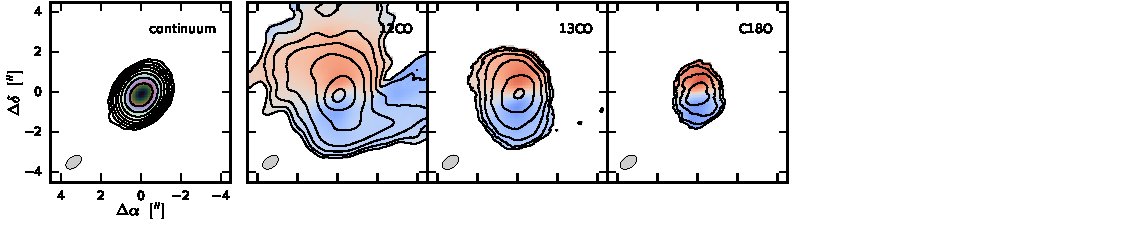
\includegraphics[width=\linewidth]{moments.pdf}
  \figcaption{({\it left}) A 226\,GHz continuum image.  Contours start at 5$\times$ the RMS noise level and increase by factors of 2.  The synthesized beam geometry is shown in the lower left corner.  ({\it middle, left to right}) Maps of the $^{12}$CO, $^{13}$CO, and C$^{18}$O velocity-integrated intensities (contours, starting at 10, 3, and 3$\times$ the RMS noise levels, respectively, and increasing by factors of 2) overlaid on the intensity-weighted projected velocities (color-scale).  Note the prominent molecular cloud contamination in the $^{12}$CO map (see also Fig.~\ref{fig:chanmaps}).  ({\it right}) Spatially integrated spectra (inside the same {\tt CLEAN} mask, and smoothed with an 0.85\,km\,s$^{-1}$ Hanning kernel) for each CO line.
  \label{fig:moments}}
  \end{center}
\end{figure*}

GW Ori was observed with the ALMA interferometer on 2015 May 14 (program ID 2012.1.00496.S), with 37 of the 12\,m main array antennas configured to span baselines of 23--558\,m.  The double sideband Band 6 receivers were employed in dual polarization mode, and the ALMA correlator was set up to process data in 4 spectral windows (SPWs).  Two of these SPWs, centered at 220.426 and 230.450\,GHz to observe the nearby $^{13}$CO and $^{12}$CO $J$=2--1 transitions (at rest frequencies of 220.399 and 230.538\,GHz, respectively), covered 234\,MHz of bandwidth in 3840 channels (a 61\,kHz channel spacing).  One other sampled 469\,MHz around 219.763\,GHz to observe the nearby C$^{18}$O $J$=2--1 transition (at rest frequency 219.560\,GHz) with 3840 channels (a 122\,kHz channel spacing).  The last SPW sampled the continuum in a 1.875\,GHz range around 231.956\,GHz using 128 coarse channels (a 15.625\,MHz channel spacing).

The observations cycled between GW Ori and the quasar J0510+1800 with a 7 minute cadence.  The quasar J0423-0120 and Ganymede were observed as bandpass and flux calibration sources, respectively, at the start of the execution block.  The total on-source integration time for GW Ori was 16 minutes.  The observing conditions were typical for Band 6 projects, with a precipitable water vapor level around 1.1\,mm.

The visibility data were calibrated with standard procedures using the {\sc CASA} software package (v4.4).  The raw, observed visibility phases were adjusted based on the contemporaneous measurements of water vapor radiometers, flagged when applicable, and then the bandpass shape in (and between) each SPW was calibrated based on the observations of J0423-0120.  The absolute amplitude scale was determined based on the observations of Ganymede.  The complex gain behavior of the array and atmosphere was corrected based on the repeated observations of J0510+1800.  The calibrated visibilities showed a strong continuum signal, suggesting that self-calibration could significantly improve the data quality.  An initial model based on a preliminary continuum image was used for two rounds of phase-only self-calibration (on 30\,s, then 6\,s intervals) and one additional round that included the amplitudes (on a 7 minute scan interval).  This self-calibration reduced the RMS noise level in the continuum by a factor of $\sim$40.  After applying the self-calibration tables to the entire dataset (channel by channel),  we parsed out data products for each individual emission tracer of interest.  A set of continuum visibilities was constructed by spectrally averaging the line-free channels in each SPW into $\sim$125\,MHz increments.  The spectral visibilities for the $^{12}$CO, $^{13}$CO, and C$^{18}$O lines were continuum-subtracted and regridded into 170\,m s$^{-1}$-wide channels in the LSRK restframe over a $\sim$10\,km s$^{-1}$ range around the line centers.

These fully reduced visibility sets were then imaged by Fourier inversion assuming a Briggs (robust=0.5) weighting scheme and deconvolution with the standard {\tt CLEAN} algorithm.  Some basic image properties for the synthesized continuum image and spectral line image cubes are listed in Table~\ref{tab:ims}.  The continuum and spectral line moment maps are shown together in Figure~\ref{fig:moments}, along with a comparison of the integrated spectra.  The channel maps for individual lines are compiled in Figure~\ref{fig:chanmaps}.

\begin{deluxetable}{lcc}[b!]
\tablewidth{18pc}
\tablecaption{ALMA Image Properties  \label{tab:ims}}
\tablehead{
\colhead{} &
\colhead{} &
\colhead{RMS}
\\
\colhead{} &
\colhead{beam dimensions} &
\colhead{mJy beam$^{-1}$}}
\startdata
226\,GHz continuum  & $0\farcs88\times0\farcs54$, 126\degr\ & 0.055 \\
$^{12}$CO $J$=2$-$1 & $0\farcs89\times0\farcs56$, 126\degr\ & 6     \\
$^{13}$CO $J$=2$-$1 & $0\farcs93\times0\farcs59$, 126\degr\ & 8     \\
C$^{18}$O $J$=2$-$1 & $0\farcs92\times0\farcs58$, 126\degr\ & 5     \\
\enddata
\tablecomments{The RMS noise levels recorded for the spectral line cubes correspond to the values per 170\,m s$^{-1}$ channel.}
\end{deluxetable}

\begin{figure*}[ht!]
\begin{center}
  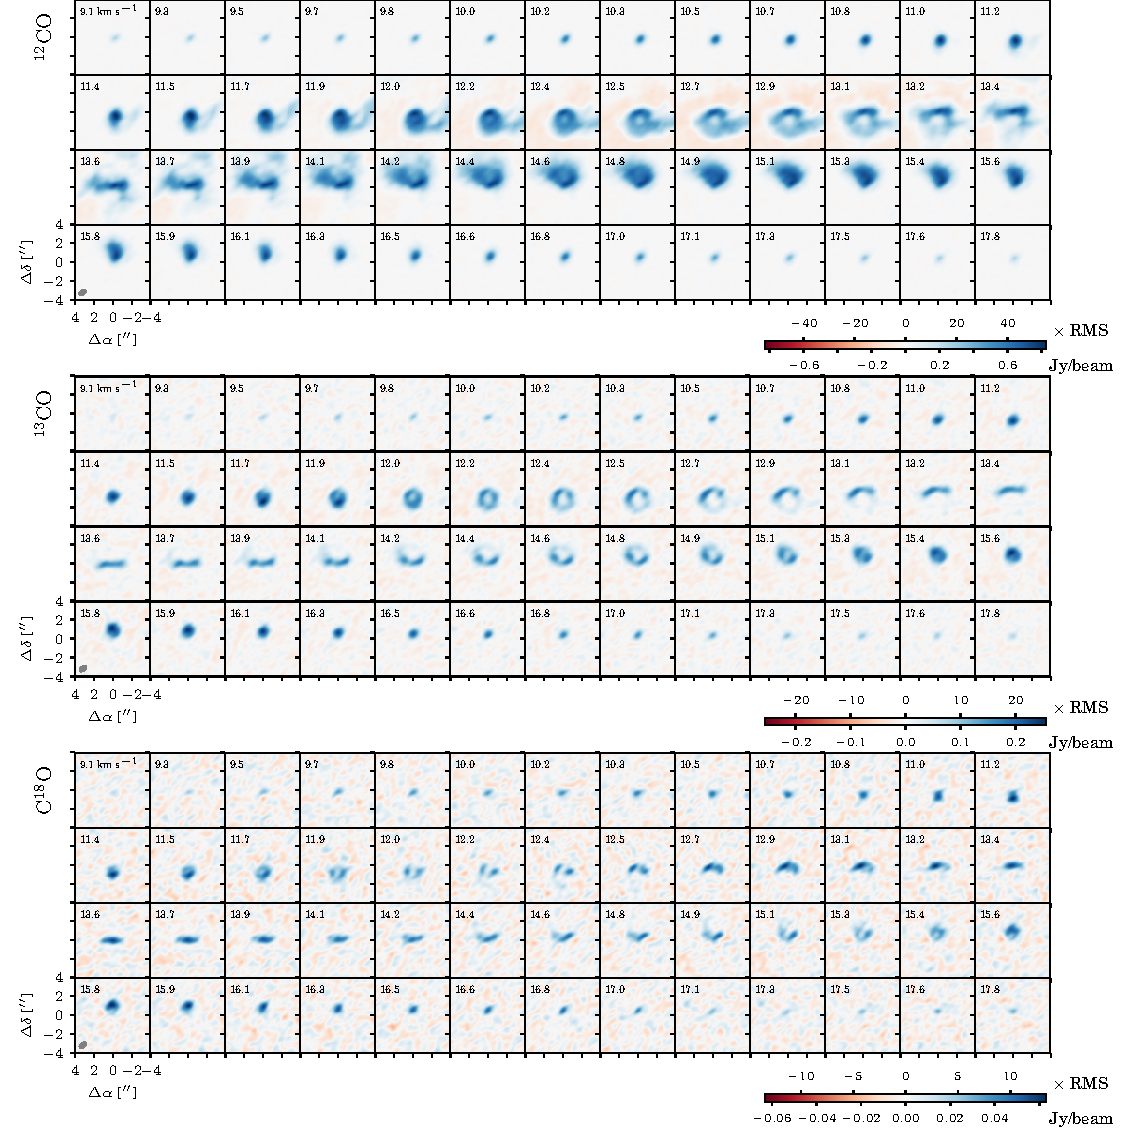
\includegraphics{chmaps_all.pdf}
  \figcaption{Channel maps of the $^{12}$CO, $^{13}$CO, and C$^{18}$O ({\it from top to bottom}) line emission from the GW Ori disk.  Each channel represents the emission in a 170\,m\,s$^{-1}$-wide velocity bin.  LSRK velocities are indicated in the upper left, and synthesized beam sizes in the lower left, or each panel.  Scale bars are provided at the bottom right of each set of channel maps.
  \label{fig:chanmaps}}
  \end{center}
\end{figure*}

The 226\,GHz (1.3\,mm) continuum map shows a bright (flux density = 202\,mJy), compact but marginally resolved (deconvolved Gaussian FWHM $\approx 0\farcs9$) source centered on the GW Ori stellar system, with a peak intensity of 67\,mJy beam$^{-1}$ (S/N $\approx 1200$). Our integrated flux density measurement is consistent with that of \citet[$255 \pm 60$\,mJy]{mathieu95},  but marginally discrepant with that of \citet[$320 \pm 64$\,mJy]{fang17}. A crude estimate of the emission geometry (from a Gaussian fit to the visibilities) suggests an inclination of 35--40\degr\ from face-on, with the major axis oriented $\sim$170\degr\ E of N.

The CO isotopologue channel maps reveal bright (integrated intensities of 41.8, 5.7, and 0.8\,Jy\,km\,s$^{-1}$ for $^{12}$CO, $^{13}$CO, and C$^{18}$O, respectively) and extended (FWHM $\sim 2\farcs5$) emission that is clearly in rotation around the continuum centroid, spanning a projected velocity range of $\pm$5\,km s$^{-1}$ from the line center.  The line emission is blueshifted to the south and redshifted to the north, consistent with the orientation estimated from the continuum emission.
The peak intensities for each line are $\sim$800, 290, and 55\,mJy beam$^{-1}$ in the brightest channels (peak S/N $\approx 130$, 35, and 14) for \twelve, \thirteen, and \eighteen, respectively. The \twelve\ channel maps show some clear evidence for structured contamination from the surrounding molecular cloud, particularly as a streamer to the west at LSRK velocities $\sim$11--13\,km s$^{-1}$ and some diffuse clumps to the north around 13--14\,km s$^{-1}$, confirming the ``tail''-like structure seen by \citet{fang17}.  These features are much fainter, but still present, in $^{13}$CO emission; they are not apparent in the C$^{18}$O maps.

\subsection{Optical Spectroscopy \label{sec:spectroscopy}}

\gw\ was monitored spectroscopically at the Harvard-Smithsonian Center for Astrophysics for more than 35 years, beginning in 1981 November. A total of 208 spectra were gathered through 2009 April using three nearly identical echelle spectrographs (Digital Speedometers, DS; now decommissioned) with a resolving power of $R \approx 35,000$ mounted on three different telescopes: the 1.5m Tillinghast reflector at the Fred L.\ Whipple Observatory (Mount Hopkins, AZ), the 4.5m-equivalent Multiple Mirror Telescope (also on Mount Hopkins) before conversion to a monolithic mirror, and occasionally on the 1.5m Wyeth reflector at the Oak Ridge Observatory (in the town of Harvard, MA).  Each instrument was equipped with an intensified photon-counting Reticon detector limiting the output to a single echelle order 45~\AA\ wide, which was centered on the region of the \ion{Mg}{1}\,b triplet at 5187~\AA\ \citep[see][]{latham92}. The signal-to-noise ratios of these observations range from 14 to 59 per resolution element of 8.5~\kms. Wavelength calibrations were based on exposures of a Thorium-Argon lamp taken before and after each science exposure. Reductions were performed with a dedicated pipeline, and the zero-point of the velocities was monitored regularly by means of exposures of the evening and morning twilight sky. A further \todo{80} spectra of \gw\ were collected with the Tillinghast Reflector Echelle Spectrograph \citep[TRES;][]{furesz08}, a bench-mounted, fiber-fed echelle instrument mounted on the 1.5m Tillinghast reflector with a resolving power of $R \approx 44,000$ and delivering 51 orders covering the wavelength interval 3900--9100~\AA. These observations were made between 2010 November and \todo{2016 April}.  Signal-to-noise ratios at 5200~\AA\ range from 28 to 195 per resolution element of 6.8~\kms. Wavelength calibration was carried out as above, and reductions were performed as described by \cite{buchhave10}. Radial-velocity standard stars were observed each night to monitor the zero point and place it on the same system as the DS observations to within $\sim$0.1~\kms.

All of our spectra appear single-lined.  Radial velocities (RVs) were measured by cross-correlation using the IRAF\footnote{IRAF is distributed by the National Optical Astronomy Observatories, which are operated by the Association of Universities for Research in Astronomy, Inc., under cooperative agreement with the National Science Foundation.} task {\tt XCSAO} \citep{kurtz98}, with templates taken from a large library of calculated spectra based on model atmospheres by R.\ L.\ Kurucz \citep[see][]{nordstroem94,latham02}.
These synthetic templates cover a 300~\AA\ region centered on the \ion{Mg}{1}\,b triplet, and are available for a wide range of effective temperatures ($T_{\rm eff}$), surface gravities ($\log g$), metallicities ([Fe/H]), and rotational broadenings ($v \sin i$ when seen in projection). The optimal template was selected by running grids of cross-correlations over broad ranges in the template parameters, as described by \cite{torres02}, seeking the best match as measured by the peak cross-correlation coefficient averaged over all exposures. This was done separately for the DS and TRES spectra, using only the order centered on the \ion{Mg}{1}\,b line, for consistency.

In principle these template parameters may be interpreted as estimates of the physical properties of the star. In practice, however, the narrow wavelength range ($\sim$100~\AA\ for TRES, 45~\AA\ for DS) limits the analysis by introducing a degeneracy between temperature, surface gravity, and metallicity such that a match of nearly equal quality is obtained by slightly increasing or decreasing these template parameters in tandem. We therefore made the reasonable assumption that \gw\ has solar metallicity, as expected for young stars, and we held $\log g$ fixed at a range of values between 2.5 and 4.0, varied in steps of 0.5, and solved only for $T_{\rm eff}$ and $v \sin i$. The best fit was found for $\log g = 3.0$, for both the DS and TRES spectra, and the resulting temperatures and rotational broadenings were very similar: 5180~K and 43~\kms\ for DS, and 5210~K and 44~\kms\ for TRES. For the remainder of the paper we adopt consensus values of $T_{\rm eff} = 5200 \pm 200$~K and $v \sin i = 44 \pm 2~\kms$.
Because of the strong dependence of temperature on the adopted surface gravity (and metallicity) we cannot rule out a bias in $T_{\rm eff}$, which may also have a contribution from veiling (not considered in our templates), if significant in the spectral region analyzed.  Radial velocities were based on a template with parameters nearest to those reported above ($T_{\rm eff} = 5250$~K, $v \sin i = 40~\kms$, $\log g = 3.0$); they are listed in Table~\ref{tab:RVs} in the heliocentric frame along with our uncertainty estimates from {\tt XCSAO}. The average internal errors for the DS and TRES velocities are 1.41 and 0.98~\kms, respectively.

\begin{deluxetable}{lcccc}
\tablewidth{18pc}
\tablecaption{Heliocentric radial velocity measurements of \gw.
\label{tab:RVs}}
\tablehead{
\colhead{HJD} &
\colhead{RV} &
\colhead{$\sigma_{\rm RV}$} &
\colhead{} &
\colhead{}
\\
\colhead{(2,400,000$+$)} &
\colhead{(\kms)} &
\colhead{(\kms)} &
\colhead{$\phi_{\rm in}$} &
\colhead{$\phi_{\rm out}$}}
\startdata
    44919.0042 &  31.43  &   1.88   &   0.2480  &  0.9360 \\
    45301.8865 &  26.55  &   1.28   &   0.8338  &  0.0274 \\
    45336.7941 &  24.43  &   1.26   &   0.9784  &  0.0358 \\
    45708.7038 &  30.41  &   1.79   &   0.5187  &  0.1246 \\
    45709.6058 &  35.22  &   1.14   &   0.5225  &  0.1248 \\
\enddata
\tablecomments{Observations up to HJD 2,454,926.6573 were obtained
  with the DS, and the remainder with TRES. Phases in the inner and
  outer orbits are represented with $\phi_{\rm in}$ and $\phi_{\rm
    out}$. This table is available in its entirety in machine-readable
  form.}
\end{deluxetable}


\subsection{Time-series Photometry}
We have assembled a $\sim$30 year high cadence lightcurve of \gw\ by drawing from several ongoing photometric surveys as well as archival observations. In this section we present the sources of our photometric data and their reduction.

\subsubsection{Maidanak Observatory}
\todo{Text from Grankin.}

\subsubsection{KELT}
The Kilodregree Extremely Little Telescope (KELT) project uses two telescopes to survey over 70\% of the entire sky searching for transiting planets around bright stars (8$<$V$<$11). The telescopes, located in Sonoita, AZ (KELT-North) and Sutherland, South Africa (KELT-South), have a 42mm Mamiya 645-series wide-angle lens resulting in a $26^{\circ}$ $\times$ $26^{\circ}$ field-of-view (FOV), and a 23$\arcsec$ pixel scale. Both telescopes use a broad $R$-band filter. KELT observes using a paramount ME German equatorial mount with a 180$^{\circ}$ meridian flip; therefore KELT observes in either a ``east'' or ``west'' orientation. The telescope optics are not perfectly axisymmetric, and so the point spread function (PSF) changes from one orientation to the other. Throughout the data reduction process, the east and west observations are treated as though they were acquired from separate telescopes. See \citet{Siverd12} and \citet{Kuhn16} for a detailed description of the KELT observing strategy and reduction process. \gw\ was located in KELT-South field 05 ($\alpha$ =  06hr 07m 48.0s, $\delta$ = $+3^{\circ}$ 00$\arcmin$ 00$\arcsec$) and was observed 2889 times from UT 2010 February 28 until UT 2015 April 09, with a median error of 0.005 mag.

\subsubsection{ASAS}
Using two observing location, in Las Campanas, Chile and Haleakala, Maui, the All-Sky Automated Survey (ASAS) project was designed to observe the entire sky to a limiting optical magnitude of 14. The two observatory setups each contained a wide-field Minolta 200/2.8 APO-G telephoto lenses with a 2K$\times$2K Apogee CCD and both observed simultaneously in $B$- and $V$-band. The telescope and camera set up correspond to a 8.8$^{\circ}\times8.8^{\circ}$ field-of-view. ASAS observed GW Ori in the $V$-band from UT 2001 March 11 until UT 2009 November 29, obtaining 480 observations with a median per-point error of 0.036 mag.

\subsubsection{ASAS-SN}
Focused on the discovery and characterization of SuperNovae, the the All-Sky Automated Survey for SuperNovae (ASAS-SN, \citet{Shappee14}) surveys the entire sky down to $V \sim 17$ mag every $\sim$2 days. Hosted by the Las Cumbres Observatory (LCO) at Mount Haleakala, Hawaii and the Cerro Tololo InterAmerican Observatory (CTIO) in Chile, each location hosts four 14-cm Nikon telephoto lenses with a 2k $\times$ 2k thinned CCD \citep{Brown13}. The telescopes have a $4.5\times4.5$ degree field-of-view and a 7$\farcs$8 pixel scale. ASAS-SN obtained 799 observations of GW Ori from UT 2014 December 16 until UT 2017 March 15, with a typical per point error of 0.01 mag.


\section{Analysis and Results}

\subsection{A Reconstruction of the Disk Velocity Field}
We use the spatially and spectrally resolved molecular line emission observed with ALMA to tomographically reconstruct the disk velocity field and make a dynamical measurement of the total stellar mass. We follow the forward modeling procedures described by \citet{czekala15a,czekala16} using the associated open-source software package {\tt DiskJockey}.\footnote{Available under an MIT license at \url{https://github.com/iancze/DiskJockey}.}

\begin{figure*}[ht!]
\begin{center}
  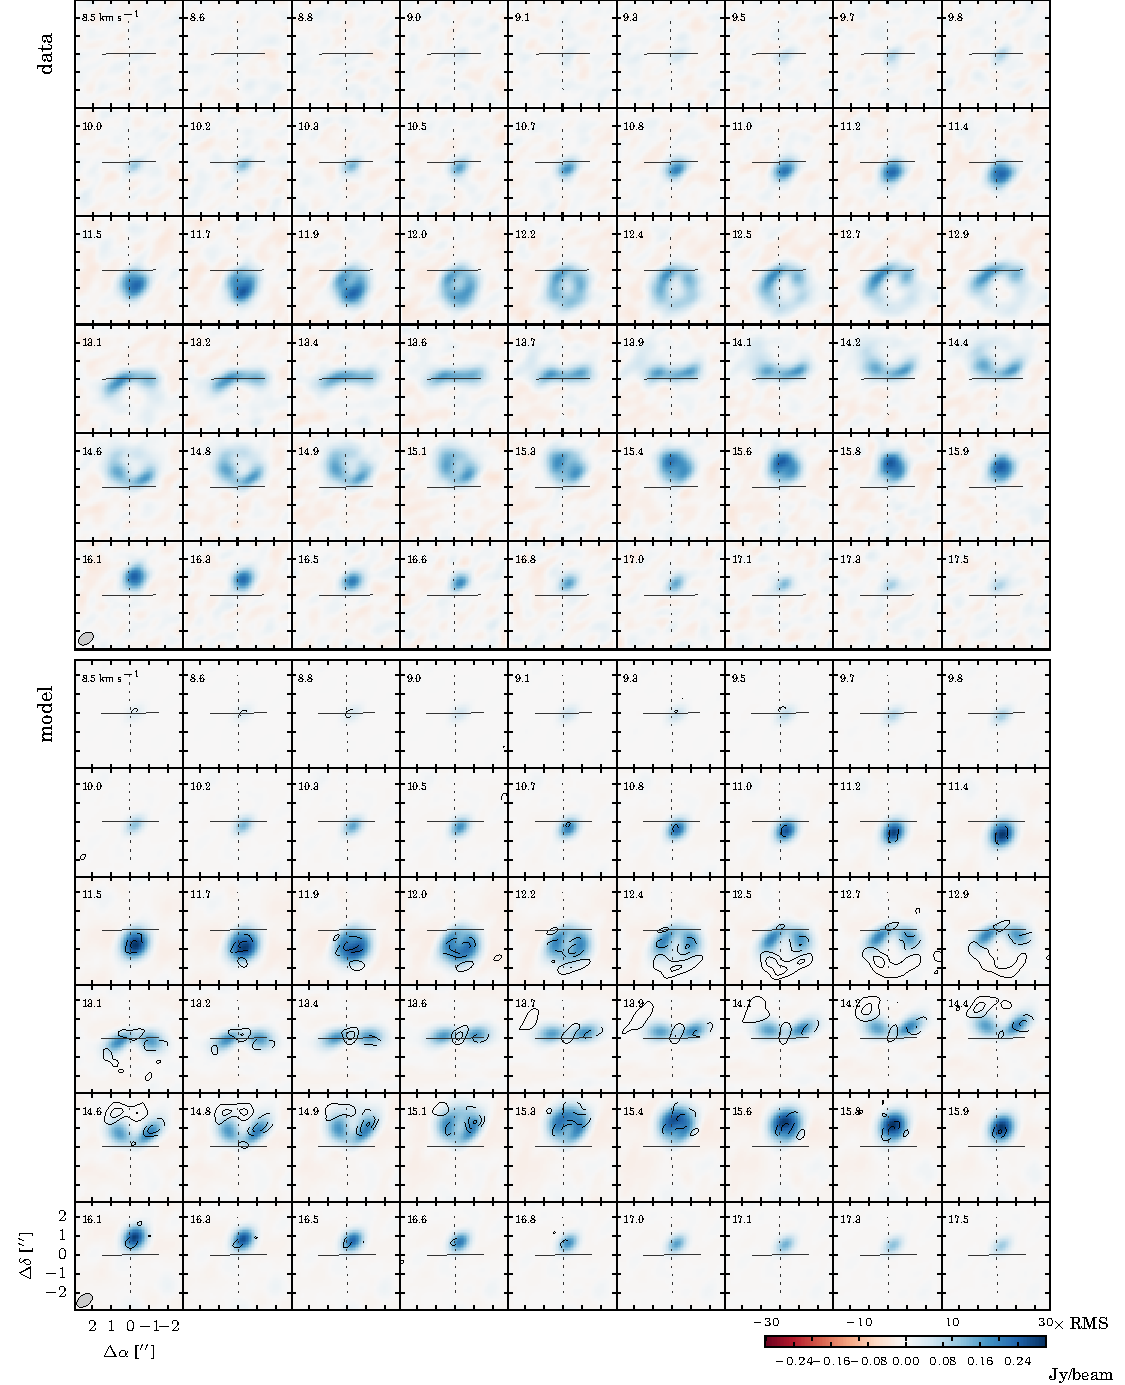
\includegraphics{chmaps_13CO.pdf}
  \figcaption{A comparison of the observed channel maps of the $^{13}$CO line emission ({\it top}) with a best-fit model ({\it middle}; constructed from a synthetic visibility set based on the inferred parameters listed in Table~\ref{table:components} and then imaged in the same way as the data) and the associated residuals ({\it bottom}; the imaged data$-$model residual visibilities).  The annotation is the same as in Fig.~\ref{fig:chanmaps}.
  \label{fig:13co}}
  \end{center}
\end{figure*}

The basis of the parametric physical model adopted in this approach is a radial surface density profile, $\Sigma(r)$, designed to mimic a simple theoretical description for a viscous accretion disk \citep{lyndenbell74,hartmann98}.  It decreases like $1/r$ interior to a characteristic radius $R_c$, and has an exponential taper $e^{-r/R_c}$ at larger radii.  The vertical distribution ($z$-direction) of these densities is controlled by the disk temperatures. To convert the total gas densities to molecule-specific values, we start with baseline abundances that are representative of the cold molecular interstellar medium: [H$_2$/ gas] = 0.8, [$^{12}$CO/H] = $7.5 \times 10^{-5}$, [$^{12}$CO/$^{13}$CO] = 69, and [$^{12}$CO/C$^{18}$O] = 557 \citep[e.g.,][]{henkel94,prantzos96}.

\begin{figure*}[ht!]
\begin{center}
  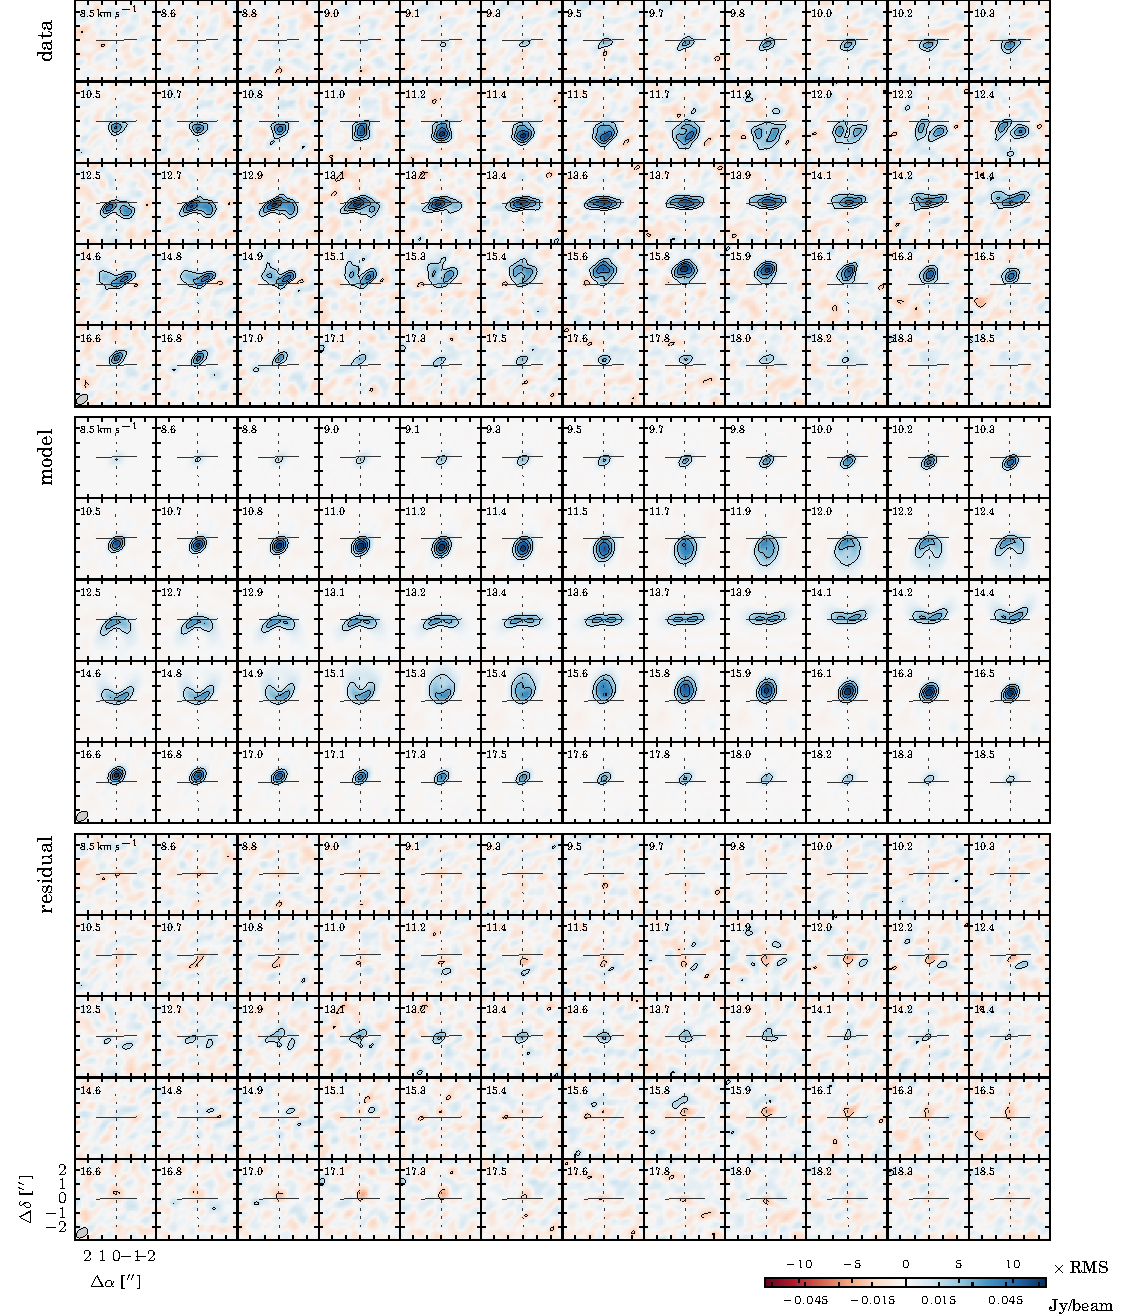
\includegraphics{chmaps_C18O.pdf}
  \figcaption{A comparison of the observed channel maps of the C$^{18}$O line emission ({\it top}) with a best-fit model ({\it middle}; constructed from a synthetic visibility set based on the inferred parameters listed in Table~\ref{table:components} and then imaged in the same way as the data) and the associated residuals ({\it bottom}; the imaged data$-$model residual visibilities).  The annotation is the same as in Fig.~\ref{fig:chanmaps}.
  \label{fig:c18o}}
  \end{center}
\end{figure*}

% We then follow \citet{qi08} to crudely account for depletions relative to these baselines associated with both photodissociation in the low-density atmosphere and freezeout onto dust grains at low temperatures.  Specifically, we set the CO abundance to zero for regions where the gas column densities (vertically integrated toward the midplane) are below $10^{20}$\,cm$^{-2}$, and we deplete the baseline abundance by a factor of 100 for the disk regions where $T<19$\,K.

The disk kinematics are assumed to be Keplerian and dominated by the total stellar mass $M_\mathrm{tot}$, with a velocity field that appropriately accounts for the two-dimensional distribution of the emitting layer \citep[see][]{rosenfeld13a}.  The  line-spread function is characterized with a width defined by the quadrature sum of thermal and non-thermal ($\xi$; presumably turbulent) contributions. For any physical structure specified by these 6 parameters, \{$\Sigma_c$, $R_c$, $T_{10}$, $q$, $M_\mathrm{tot}$, $\xi$\}, we solve the molecular rate equations (assuming LTE) and ray-trace the associated emission into a set of high resolution channel maps using the radiative transfer package {\tt RADMC-3D} \citep{dullemond12}.
That ray-tracing requires that we specify 3 additional geometric parameters: the disk inclination to the line-of-sight ($i_\mathrm{disk}$), the position angle of the disk rotation axis projected on the sky ($\varphi$), and the LSRK systemic radial velocity ($v_r$). Hereafter, we term this parameterization the ``standard'' model. The model channel maps are then Fourier transformed and sampled at the same spatial frequencies observed by ALMA.  The model quality with respect to the observed visibilities is evaluated with a $\chi^2$ likelihood function that incorporates the nominal visibility weights.
We assume flat priors on all parameters except for $i_\mathrm{disk}$, where we adopt a simple geometric prior \citep[the disk angular momentum vector
${\bm h}_\mathrm{disk}$ is distributed uniformly on a sphere, e.g.;][]{czekala16}. We adopt a fixed distance to GW Ori of $d = 388\,$pc \citep{kounkel17} to make the problem more computationally tractable; we discuss the effects of this assumption in Section~\ref{sec:joint}. The posterior distribution of these parameters is explored using Markov Chain Monte Carlo simulations with the affine invariant ensemble sampler proposed by \citet{goodman10}, as implemented in the {\tt emcee} code \citep{foreman-mackey13} and ported to the {\tt Julia} programming language, which we include in {\tt DiskJockey}.

\begin{deluxetable}{lcc}
\tablecaption{Inferred Disk Model Parameters\label{table:components}}
\tablehead{\colhead{Parameter} & \thirteen & \eighteen}
\startdata
$M_\ast\quad [M_\odot]$ & $5.28 \pm 0.06$ & $5.38 \pm 0.23$ \\
$r_c$ [au] & $237 \pm 5$ & $151 \pm 21$ \\
$T_{10}$ [K] & $51 \pm 2$ & $32 \pm 4$ \\
$q$ & $0.308 \pm 0.012$ & $0.378 \pm 0.037$ \\
$\log_{10} M_\mathrm{disk} \quad \log_{10} [M_\odot]$ & $-1.69 \pm 0.02$ & $-1.02 \pm 0.22$ \\
$\xi\,[\kms]$ & $0.59 \pm 0.01$ & $0.37 \pm 0.03$ \\
$i_d \quad [{}^\circ]$ & $137.7 \pm 0.3$ & $135.2 \pm 1.4$ \\
PA\tablenotemark{a} $[{}^\circ]$ & $90.7 \pm 0.1$ & $90.5 \pm 0.6$ \\
$v_r\,[\kms]$ & $13.651 \pm 0.003$ & $13.649 \pm 0.015$ \\
$\mu_\alpha\,['']$  & $-0.004 \pm 0.002$ & $-0.028 \pm 0.010$ \\
$\mu_\delta\,['']$ & $-0.044 \pm 0.002$ & $-0.051 \pm 0.008$ \\
\enddata
\tablenotetext{a}{For comparison with the stellar orbits, we note that the position angle of the ascending node $\Omega_\mathrm{disk}$ is $90^\circ$ offset from our PA convention, i.e. $\Omega_\mathrm{disk} = \mathrm{PA} + 90^\circ \approx 180.6^\circ$.}
\tablecomments{The 1D marginal posteriors are well-described by a Gaussian, so we report symmetric error bars here.}
\end{deluxetable}

Compared to our previous similar work, the modeling of \obj\ is considerably more computationally intensive. This is primarily a consequence of the large physical size of the disk, which makes the ray-tracing step substantially more time-consuming. The inference for an individual spectral line takes $\sim$10,000 CPU hours parallelized across 26 cores on the Harvard Odyssey Cluster.  Given that restriction and the fact that the $^{12}$CO line is clearly contaminated by local cloud material, we restrict our analysis to {\it independent} inferences of the model parameters based on the $^{13}$CO and C$^{18}$O data only. For computational expediency we only model the data averaged to 25 channels of $0.4\,\kms$ width. Experiments modeling a subset of the channels at higher resolution (e.g., every third channel) did not yield a significantly different result.

\begin{figure*}[ht!]
\begin{center}
  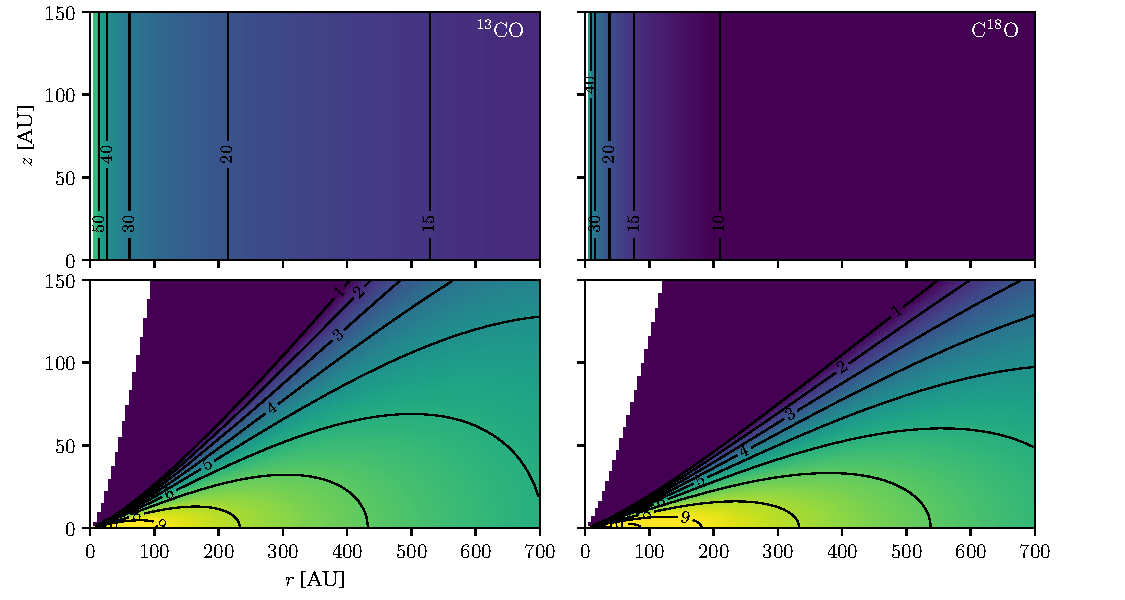
\includegraphics{temperature_and_density.pdf}
  \figcaption{The maximum likelihood 2D temperature (top) and density (bottom) disk structures inferred using the \thirteen\ (left) and \eighteen\ (right) transitions. The temperature contours are in units of K. The density plots show the total gas density ($\rho_\mathrm{gas}$) and are in units $\log_{10} \mathrm{cm}^{-3}$. The color scales are normalized to the same limits for both transitions.
  \label{fig:temp_dens}}
  \end{center}
\end{figure*}

\begin{figure}[ht!]
\begin{center}
	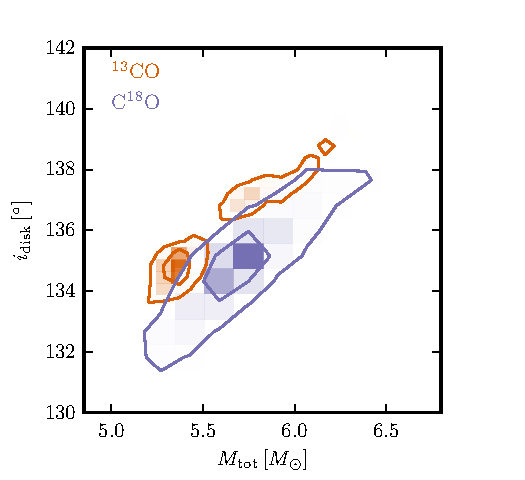
\includegraphics{posterior.pdf}
  \figcaption{Posterior distributions for the model parameters fit to the \thirteen\ and \eighteen\ data independently, showing 1 and 2 $\sigma$ contours. Dashed lines indicate constant values of $M_\mathrm{tot} \sin^2 i_\mathrm{disk}$. \label{fig:posterior}}
  \end{center}
\end{figure}

The inferred parameter values corresponding to the measurements of each spectral line are summarized together in Table~\ref{table:components}.  A comparison of the data and the best-fit models (and associated residuals) is presented in the form of channel maps in Figures~\ref{fig:13co} and \ref{fig:c18o} for $^{13}$CO and C$^{18}$O, respectively.  While overall the models successfully reproduce the observed emission, there are some interesting residuals. Namely, an excess of emission in the center of the disk for the channels between $13.1 - 14.3\,\kms$, seen in both \thirteen\ and \eighteen. We will return to a discussion of a potential origin in Section~\ref{sec:discussion}.

Motivated by the presence of the aforementioned residuals, we explored more sophisticated disk models, including a model with a vertical temperature gradient and CO depletion due to freeze-out and photodissociation \citep[after][]{rosenfeld13a}, as well as a flexible temperature model parameterized to mimic more sophisticated (and computationally expensive) protoplanetary disk models \citep{kamp04,jonkheid04}. However, we found that neither of these models resulted in a more satisfactory fit to the data as measured by visual inspection and the Akaike information criterion (AIC). Encouragingly, however, they still yielded similar estimates of $M_\mathrm{tot}$ as the standard model, which gives us confidence that the disk-based dynamical mass is moderately robust to choice of parameterization for the temperature and density structures.

Using the standard model, the inferred physical structures inferred from each line are in mild disagreement, as might be expected for this simple parameterization. To illustrate these differences, we plot the 2D temperature and density profiles inferred from each transition in Figure~\ref{fig:temp_dens}. We attribute these differences to the different layers of the disk probed by the \thirteen\ and \eighteen\ transitions. In Figure~\ref{fig:posterior}, we plot the marginalized posteriors for both transitions in the \{$M_\ast$, $i_\mathrm{disk}$\}-plane. Interestingly, the different transitions deliver different inclinations at a statistically significant level ($\Delta i_\mathrm{disk} \approx 2.5^\circ$), which we attribute to the previously mentioned model deficiencies and the fact that the \thirteen\ and \eighteen\ transitions probe different layers in the disk.
This difference is potentially concerning because biases in the measurement of disk inclination have the greatest potential to affect the inference of $M_\mathrm{tot}$. With more computational power, it would be worthwhile to explore a joint fit to both transitions, to see if a single disk structure could adequately fit both transitions simultaneously.
Nevertheless, both transitions yield consistent constraints on the total stellar mass, which is the most relevant parameter to our stated goals. We believe that the robustness of the dynamical mass technique is primarily because the kinematic morphology of the line emission (i.e., the location of the emission in R.A., Dec., and radial velocity space) is not strongly dependent on the exact temperature and density structure of the disk, but is rather a strong function of $M_\mathrm{tot}$ and $i_\mathrm{disk}$, and when the disk is spatially resolved, the dependence on $i_\mathrm{disk}$ is diminished. We combine the inferred total masses from \thirteen\ and \eighteen\ in a weighted mean to get $M_\mathrm{tot} = 5.29 \pm 0.06\,M_\odot$.
The uncertainty in the distance to \gw\ \citep[$388 \pm 5\,$pc;][]{kounkel17} linearly translates into a mass uncertainty, and so we convolve an additional 1.3\% mass uncertainty with this posterior to get  $M_\mathrm{tot} = 5.29 \pm 0.09\,M_\odot$, which we adopt as our reported total mass estimate. Because the inferred disk inclinations are mutually inconsistent, we adopt a weighted average for the mean inclination and assume a large systematic uncertainty, resulting in a final estimate of $i_\mathrm{disk} = 137.6 \pm 2.0^\circ$. Our CO results are broadly consistent with that determined by \citet{fang17}, who measure the disk inclination to be $\sim 35^\circ$.

% they say the disk inclination is ~35 degrees. We also slightly disagree with this, since we have i = 137 degrees = 43 degrees. This is close enough, though.
% Fang determines the disk is in Keplerian rotation, due to analysis of the 12CO maps. Substantial inclination to our line of sight.
% From the 12CO modeling, they get i = 40 degrees, and PA = 10 degrees. The PA convention must be offset from us, so its discrepancy is actually somewhat significant (we determine 90 degrees, so this is 10 degrees offset).
% Fit the 12CO only. Then they see that 13CO agrees, but C18O is too faint by a factor of three. Dust absorption of the line emission could be a factor


\begin{figure*}
\begin{center}
  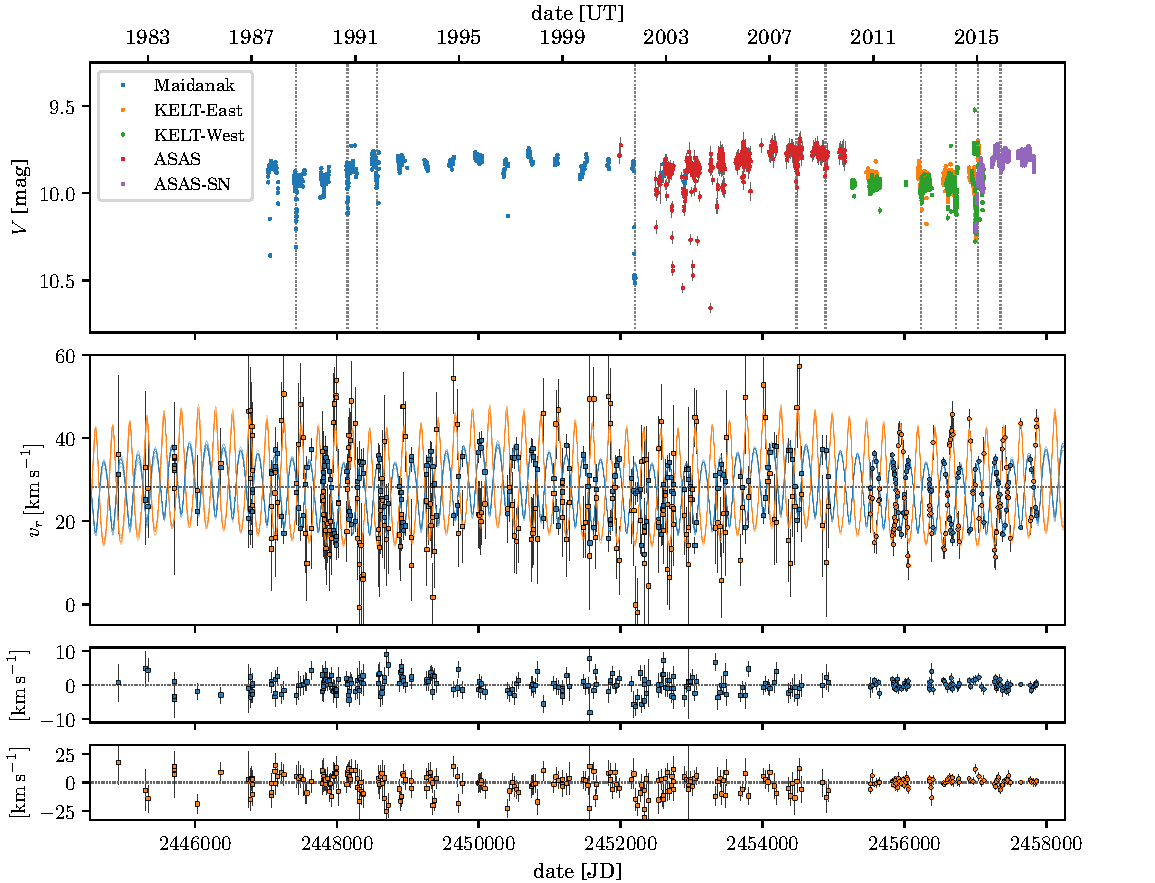
\includegraphics{lightcurve-rv.pdf}
  \figcaption{Figures for the lightcurve and radial velocities. Radial-velocity measurements of \gw\ as a function of time, and best-fit model for the triple system. The dotted line represents the center-of-mass velocity. The KELT East (black), KELT West (blue), ASAS (red), ASAS-SN (purple), and $V$-band observations from Grankin et al. (yellow) photometric observations of GW Ori from 1987 until mid 2017. All photometric observations displayed here are in the $V$-band (ASAS, ASAS-SN, and Grankin et al.) or a broader filter (KELT). To place all photometric data on the same scale, we assume the $V$-band observations as the photometric standard and apply a vertical offset to the KELT observations to align them where they overlap. We do not otherwise correct for the filter differences. The gray vertical lines represent the time of the identified eclipses.
  \label{fig:orbitboth}}
\end{center}
\end{figure*}

\begin{figure}[!ht]
\centering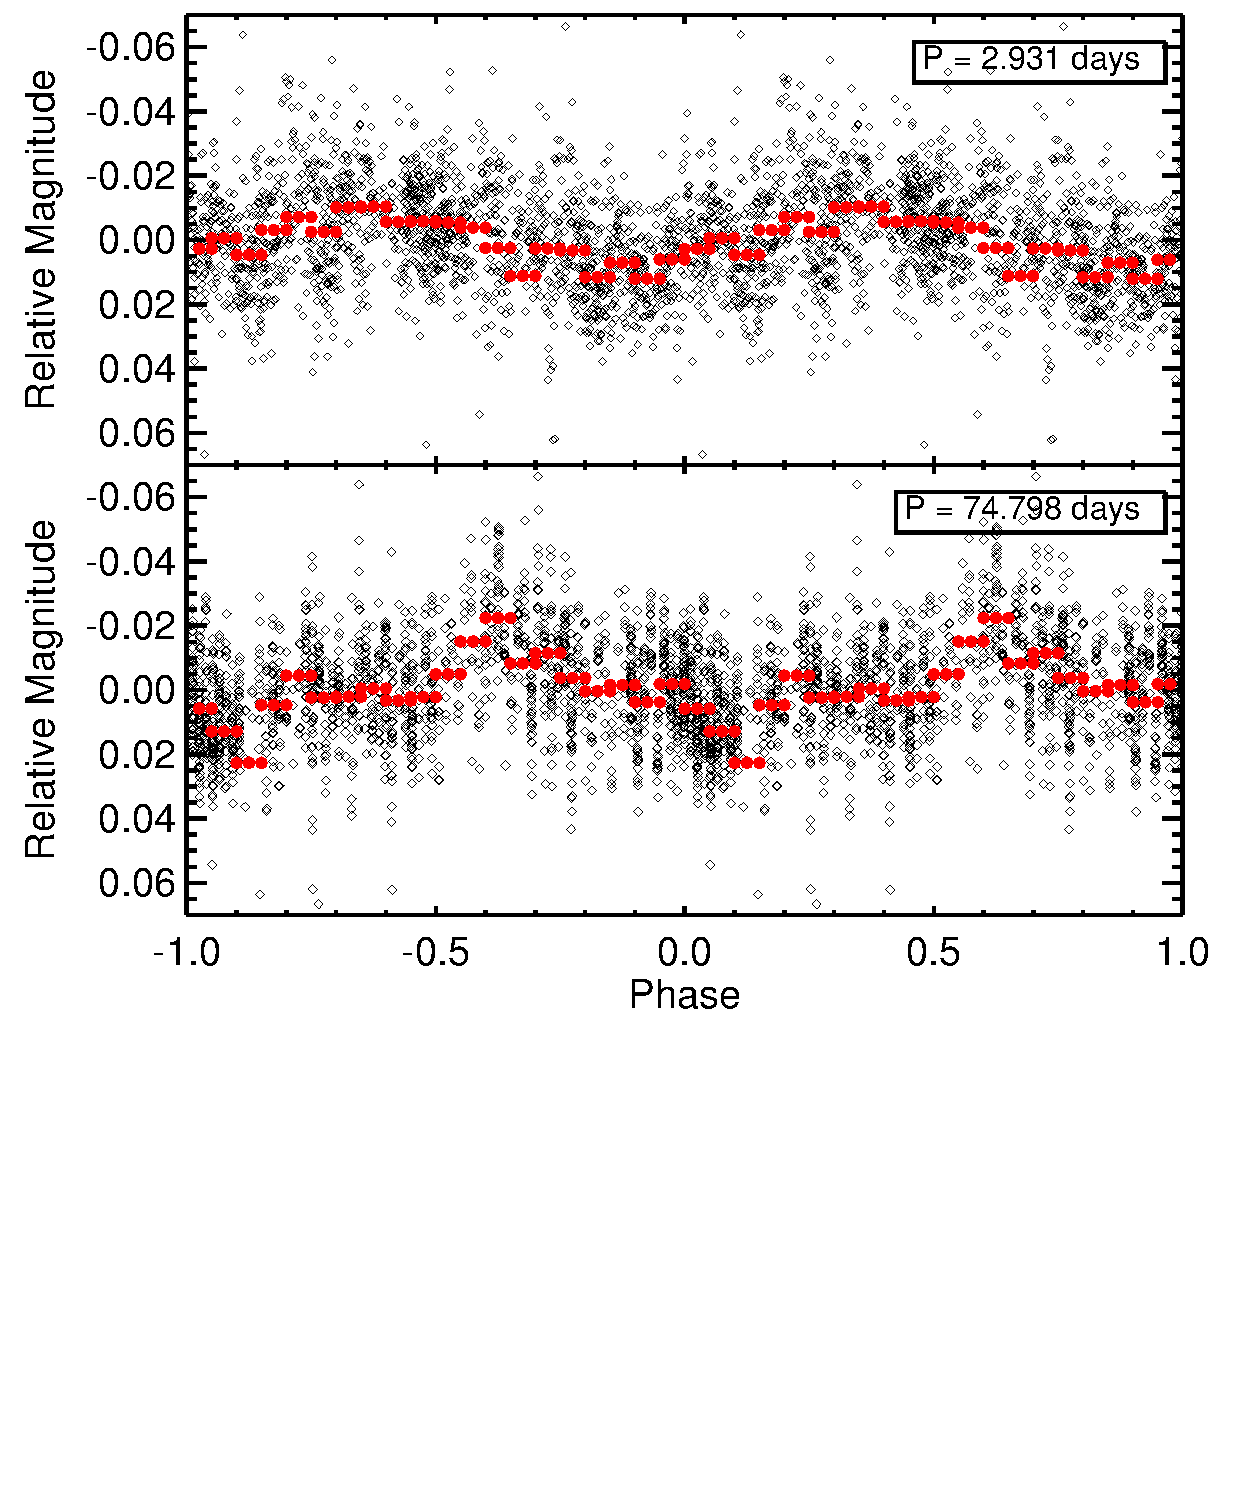
\includegraphics[width=0.99\linewidth, trim = 0 3.5in 0 0]{Figure_Phased.pdf}
\caption{The KELT photometric observations of GW Ori, with the three eclipses removed, phased to the 2.931 (Top) and 74.798 (Bottom) day periods recovered from our LS analysis. }%The red line represents a simple sinusoidal fit to the phased lightcurve.}
\label{figure:phased}
\end{figure}


\begin{figure}
\begin{center}
  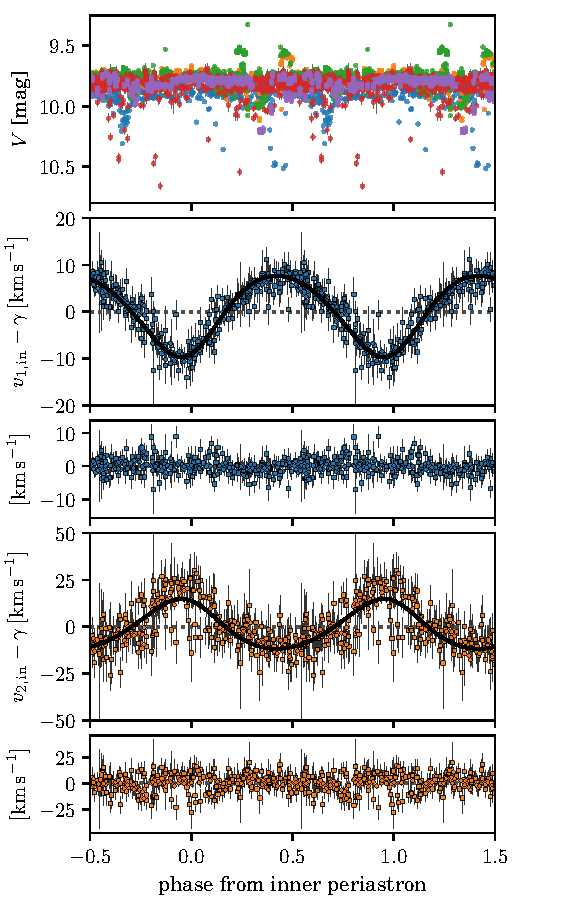
\includegraphics{inner-orbit.pdf}
  \figcaption{Radial-velocity measurements of \gw\ and best-fit model for the inner orbit, after subtracting the motion in the outer orbit. The dotted line in the top panel represents the center-of-mass velocity of the triple system. The bottom panel displays the residuals.
  \label{fig:orbitin}}
\end{center}
\end{figure}

\begin{figure}
\begin{center}
  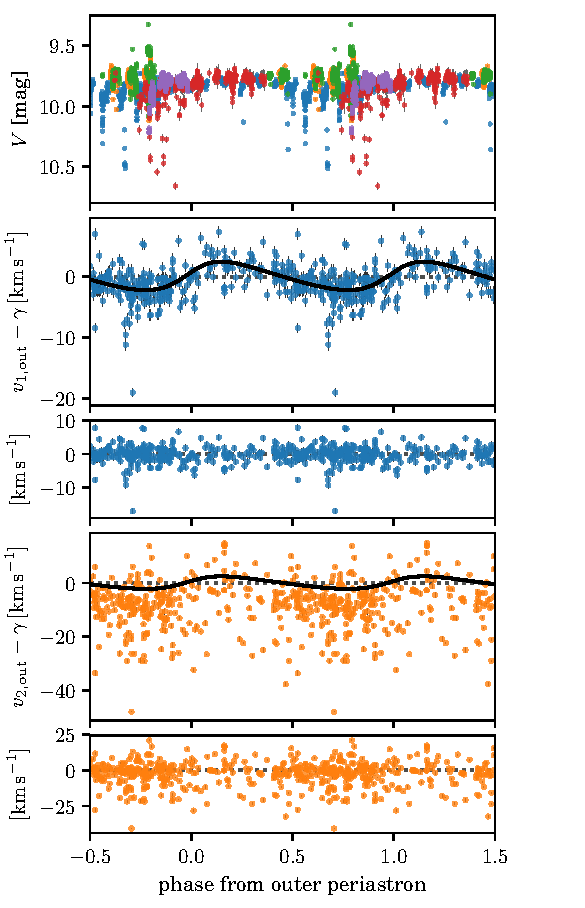
\includegraphics{outer-orbit.pdf}
  \figcaption{Radial-velocity measurements of \gw\ and best-fit model for the outer orbit, after subtracting the motion in the inner orbit. The dotted line in the top panel represents the center-of-mass velocity of the triple system. The bottom panel displays the residuals. The ASAS (red), ASAS-SN (purple), and Maidanak (yellow) $V$-band photometric observations of GW Ori phased to $\sim$4121 days, the derived orbital period of the outer companion.
  \label{fig:orbitout}}
\end{center}
\end{figure}

\subsection{An Updated Model of the Stellar Orbits} \label{sec:orbit}
The discovery orbit of \gw\ by \cite{mathieu91}, with a period of 242 days, was based on a small subset of the same spectra used here, covering slightly more than seven years. The present data set is six times larger and extends the time coverage to nearly 35 years. \cite{mathieu91} noted a drift in the residuals from their spectroscopic orbit that they speculated could be due to a third component, or perhaps an asymmetry in a massive circumbinary disk,
causing the reflex motion of the inner binary with a period exceeding their time coverage. As our data set expanded over the years, our own preliminary spectroscopic solutions for the 242-day orbit displayed an
increasingly clear periodic pattern in the residuals with a period of about 11.5 years, strongly suggesting the presence of a third body in the \gw\ system with a nearly circular orbit. Direct near-infrared
imaging by \cite{berger11} revealed the stellar nature of the third component for the first time, and also resolved the inner binary. Given the moderate H-band flux ratio that \citet{berger11} found between the primary and secondary, we began searching for spectroscopic signatures of the secondary.

After experimenting with spectroscopic disentangling techniques (see \S\ref{sec:psoap}) and learning that spectroscopic light from the secondary was successfully detected with high resolution infrared spectra (L. Prato, private communication, March 2017), we refocused our efforts on splitting the cross-correlation function via traditional \texttt{TODCOR} techniques. Our extended time coverage in radial velocities now enables us to derive robust spectroscopic orbits for the second and third stars.

We fit a hierarchical triple orbit and solve for the elements of the inner and outer Keplerian orbits simultaneously, assuming the inner binary acts as a point mass in the outer orbit. The residuals from our initial fit indicated our formal velocity errors are slightly underestimated, so for our final solution we have used a likelihood function.

The period of the inner orbit is consistent with that of \cite{mathieu91}, and the eccentricity is insignificant, as was
also found by them. On the other hand, the velocity semi-amplitude of our inner orbit, $K_{\rm A} = 3.54 \pm 0.11~\kms$, is significantly smaller than theirs ($K_{\rm A} = 4.7 \pm 0.3~\kms$), but similar to the one by \cite{fang14} ($K_{\rm A} = 3.41 \pm 0.17~\kms$). Graphical representations of our observations and the inner and outer
orbit models as a function of orbital phase are shown in Figure~\ref{fig:orbitin} and Figure~\ref{fig:orbitout}, respectively, and a representation of the full motion as a function of time is seen in Figure~\ref{fig:orbitboth}.

Due to the uncertainty in measured radial velocities due to the unknown flux ratio, we explore radial velocity fits using a ``robust'' likelihood advocated by \citet[Sec. 8.3.1]{sivia06} as a conservative formulation for cases where the quoted uncertainty on each data point (in this case, the statistical errors from the \texttt{TODCOR} RV analysis) are treated as lower limits on the actual uncertainty, and have the possibility of growing by some scale factor. This likelihood has wider ``tails'' than the Gaussian likelihood function used in $\chi^2$ analysis, and is less sensitive to outliers at a (minor) expense of statistical power to constrain the orbital parameters. Given the large residuals from the orbital fit, we conclude that the statistical uncertainty of each measurement is an underestimate of the true uncertainty, and that there is a large contribution from unknown systematic effects and that a more robust likelihood function is warranted until the sources of the systematic errors can be identified.

Although there are only three epochs of published astrometry in \citet{berger11}, these points may still considerably constrain the parameter space of possible orbits. Therefore, we explore a joint RV-astrometric analysis built upon a model of the ``three-dimensional orbit'' following \citet{murray10}, which adds new model parameters like the semi-major axis, inclination, and position angle on the sky for both inner and out orbits. For a likelihood function, we use a combination of the aforementioned robust likelihood for the radial velocity measurements and a $\chi^2$ likelihood function for the separation and azimuth measurements.
As with the disk analysis, we also use a geometric prior on the orbital inclinations.
The newly constrained parameters are in Table~\ref{tab:elements}. The stellar components are $M_A = 3.24 \pm 0.40\,M_\odot$, $M_B = 1.56 \pm 0.20\,M_\odot$, $M_C = 0.76\pm 0.22\,M_\odot$, and the total mass is $M_\mathrm{tot} = 5.26 \pm 0.55$, which is nicely consistent with that independently measured by the disk-based analysis.

The derived elements of the inner and outer orbits are presented in Table~\ref{tab:elements}, along with other properties derived from them.

\begin{deluxetable*}{lcc}
\tablewidth{0pc}
\tablecaption{Orbital elements of \gw. \label{tab:elements}}
\tablehead{
\colhead{~~~~~~~~~~~~Parameter~~~~~~~~~~~~} & \colhead{RV} & \colhead{RV + astrometry}
}
\startdata
\multicolumn{3}{c}{Inner orbit} \\
\noalign{\vskip 1pt}
\noalign{\hrule}
\noalign{\vskip 3pt}
$P$ [days]\dotfill                        &    241.446~$\pm$~0.066\phn\phn  & \\
$\gamma$ [\kms]\dotfill                   &    +27.726~$\pm$~0.082\phn\phs & \\
$\Delta v_\mathrm{B}$\tablenotemark{a} [\kms] \dotfill & ? & \\
$K_\mathrm{A}$ [\kms]\dotfill                 &        3.54~$\pm$~0.11 & \\
$q$ \dotfill & & \\
$e$\dotfill                               &      0.016~$\pm$~0.029 & \\
$i$ [deg] \dotfill & \nodata & \\
$\omega_\mathrm{A}$ [deg]\dotfill                    &        210~$\pm$~100 & \\
$\Omega$\tablenotemark{b} [deg]\dotfill                    &  \nodata      & \\
$T_{\rm peri}$ [HJD$-$2,400,000]\dotfill   &      51861~$\pm$~67\phm{222} & \\
$M_\mathrm{A}$ [$M_{\odot}$] \dotfill & \nodata & \\
$M_\mathrm{B}$ [$M_{\odot}$] \dotfill & \nodata & \\
\noalign{\vskip 2pt}
\noalign{\hrule}
\noalign{\vskip 2pt}
\multicolumn{3}{c}{Derived properties from inner orbit} \\
\noalign{\vskip 1pt}
\noalign{\hrule}
\noalign{\vskip 3pt}
$a_{\rm A} \sin i$ [au]\dotfill   &      0.0787~$\pm$~0.0024\phn & \\
$f(M)$ [$M_{\sun}$]\dotfill                &    0.00111~$\pm$~0.00010 & \\
$M_{\rm B} \sin i /(M_A + M_B)^{2/3} \;$[$M_{\sun}$]\dotfill            &     0.1036~$\pm$~0.0031 & \\
Time interval [days]\dotfill              &            12574 & \\
Time interval [cycles]\dotfill            &             52.1 & \\
\noalign{\vskip 2pt}
\noalign{\hrule}
\noalign{\vskip 2pt}
\multicolumn{3}{c}{Outer orbit} \\
\noalign{\vskip 1pt}
\noalign{\hrule}
\noalign{\vskip 3pt}
$P$ [days]\dotfill                        &       4187~$\pm$~42\phn\phn & \\
$K_{\rm AB}$ [\kms]\dotfill                &       2.04~$\pm$~0.12 & \\
$e$\dotfill                               &      0.061~$\pm$~0.058 & \\
$i$ [deg] \dotfill & \nodata & \\
$\omega_\mathrm{AB}$ [deg]\dotfill                    &        276~$\pm$~48\phn & \\
$\Omega$\tablenotemark{b} [deg]\dotfill                    &    \nodata    & \\
$T_{\rm peri}$ [HJD$-$2,400,000]\dotfill   &      53560~$\pm$~565\phn\phn & \\
$M_\mathrm{C}$ [$M_{\odot}$] \dotfill & \nodata & \\
\noalign{\vskip 2pt}
\noalign{\hrule}
\noalign{\vskip 2pt}
\multicolumn{3}{c}{Derived properties from outer orbit} \\
\noalign{\vskip 1pt}
\noalign{\hrule}
\noalign{\vskip 3pt}
$a_{\rm AB} \sin i$ [au]\dotfill  &      0.782~$\pm$~0.045\phn\phn & \\
$f(M)$ [$M_{\sun}$]\dotfill                &    0.00364~$\pm$~0.00062 & \\
$M_{\rm C} \sin i / (M_\mathrm{tot}\tablenotemark{c} / M_\odot)^{2/3} \; $[$M_{\sun}$]\dotfill            &     0.1539~$\pm$~0.0088 & \\
Time interval [cycles]\dotfill            &             3.0 & \\
\enddata
\tablenotetext{a}{We fit for a possible velocity offset  between the primary and secondary radial velocities. In reality, this term should be $0$, however, the non zero value likely indicates that there may be a degree of template mismatch between the stellar spectra and the synthetic spectra used as cross correlation templates.}
\tablenotetext{b}{We follow the convention of the visual binary field and define the ascending node as the line of nodes where the secondary component (e.g., star B for the inner orbit, and star C for the outer orbit) crosses the plane of the sky moving \emph{away} from the observer.}
\tablenotetext{c}{$M_\mathrm{tot} = M_\mathrm{A} + M_\mathrm{B} + M_\mathrm{C}$.}
% \tablecomments{}
\end{deluxetable*}


\begin{figure*}[ht!]
\begin{center}
  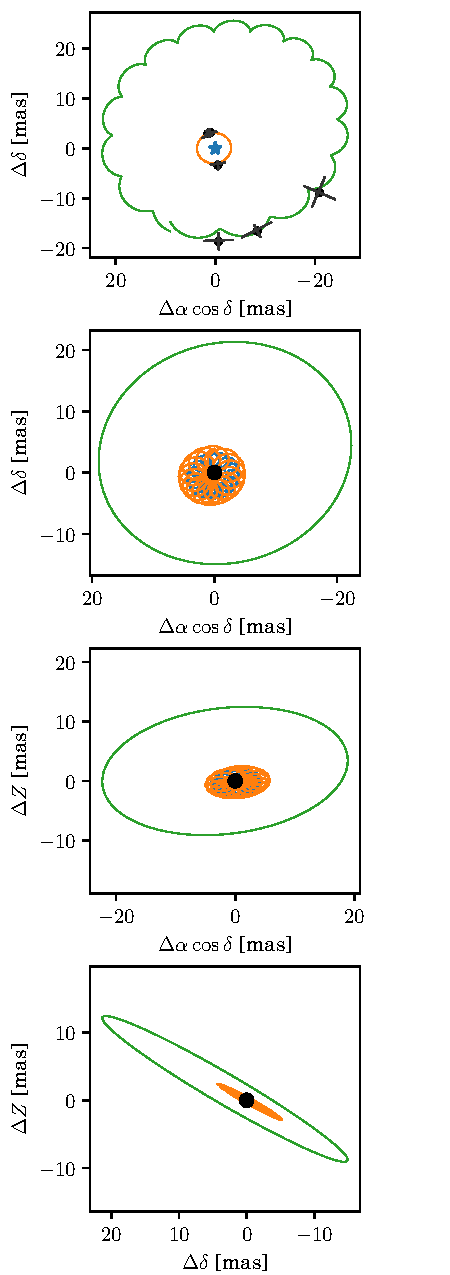
\includegraphics{astro.pdf}
  \figcaption{Orbits from the joint RV-astrometric fit. Orbits are shaded according to their phase, where black represents periastron and color hue increases with orbital phase. \emph{top left}: orbits relative to the primary star A, in the plane of the sky, with the three epochs of astrometry from \citet{berger11}. \emph{top right}:, sky plane, relative to center of mass. Bottom left, looking down North axis. Bottom right, looking down East axis.
  Positive Z axis points towards observer.
  Representative circular disk orbit shown as grey dashed line.
  \label{fig:astro}}
\end{center}
\end{figure*}

Interestingly, the inner orbital plane is inferred to be misaligned with the circum-triple disk at a statistically significant level ($i_\mathrm{disk} \approx 137^\circ$, $\Omega_\mathrm{disk} \approx 180.6^\circ$), and the outer orbital plane also appears to be inconsistent with the disk inclination, as well. Using our radial velocity results and a wide range of permissible orbital elements, one would infer that at the first epoch (2003) of the \citet{berger11} astrometric measurements the tertiary would be moving with a large positive radial velocity (relative to the systemic velocity) and by the last epoch (2005) it would be moving at approximately the systemic velocity, suggesting that the line of nodes for the outer orbit is close to the E-W axis.
Meanwhile, our disk results clearly demonstrate that the line of nodes for the disk is the N-S axis, suggesting that these orbits must be misaligned. We note that both of these claims of misalignment rest upon only three astrometric epochs, however, so we caution against overinterpretating the exact results. In the next section, we use only our newly derived radial velocity and disk modeling results to form a more conservative estimate of the relative inclinations, but also find strong evidence that the inner stellar orbit and disk are at least mildly misaligned. We advocate future astrometric monitoring of the \gw\ system to further improve the three-dimensional orbit and confirm the inclinations of the stellar orbits.

\subsection{Disentangling the \gw\ Double-lined Spectroscopic Binary}
At optical wavelengths, \gw\ clearly appears to be a \emph{single}-lined spectroscopic binary, despite full coverage of the 240 day inner period at moderate to high SNR \citep{mathieu91,fang14}. In this context, the \citet{berger11} H-band detections of the secondary and tertiary stars at favorable flux ratios ($f_B / f_A = 0.57 \pm 0.05$, and $f_C / f_A = 0.23 \pm 0.01$) were rather puzzling, since such a bright secondary companion should have detectable signatures in the optical spectra. We originally embarked on a search for these signatures using the then-under-development \texttt{PSOAP} spectroscopic disentangling package \citep{czekala17}, with a strong assumption that these spectral signatures must be at or near the detection limit (e.g., $q_\mathrm{in} \lesssim 0.2$), since they had not been seen in previous analyses. Our preliminary results hinted at the detection of a secondary spectrum, but with mass ratios much larger than what we had expected ($q_\mathrm{in} > 0.5$). Because the code was still under development at that time, we discounted these initial results as spurious and possibly the result of contamination by stellar variability.
To our excitement, however, shortly thereafter we learned that \gw\ had been revealed as a \emph{double}-lined spectroscopic binary using targeted high resolution infrared spectroscopy (L. Prato, private communication, March 2017), but at a much larger mass ratio than we had assumed ($q_\mathrm{in} \sim 0.65$). Using this knowledge, we renewed our efforts to search for the secondary signature using \texttt{PSOAP} and targeted \texttt{TODCOR} analysis.


The \texttt{PSOAP} spectroscopic disentangling technique works as an inference framework. Given a time-series of high resolution spectroscopic observations covering the orbital phase of the binary or triple star, it simultaneously infers the intrinsic spectrum of each star along with the stellar orbit (the radial velocity of each star as a function of time). \texttt{PSOAP} uses Gaussian processes to model the unknown stellar spectra, providing a robust probabalistic framework by which the spectra and orbits can be inferred in a purely data-driven manner. Once disentangled, these spectra can be used to infer fundamental stellar properties by traditional analysis techniques. For more information on the mathematical details on \texttt{PSOAP} please consult \citet{czekala17}. At present, one limitation of the \texttt{PSOAP} framework (and Gaussian processes in general, to some extent) is the heavy computational requirement for performing the matrix calculations. This generally limits us to considering less than 20 epochs of high resolution spectra at a time.

Consequentially, this limits the complexity of the orbital model that we can use. Although it was straightforward to extend the framework to utilize a hierarchical triple orbital model and three Gaussian process components, we found that we were unable to employ enough spectroscopic epochs to sufficiently constrain the more complex orbital model. Therefore, we experimented using different subsets of the data to test our sensitivity to presence of secondary and tertiary spectral signatures. In all of these tests, we clearly detected the features of the secondary but found no solid evidence for visible spectroscopic signatures of the tertiary. We have identified possible avenues of development to expand the number of spectroscopic epochs under consideration, but this will require more development and testing beyond the scope of this paper.


While \texttt{PSOAP} unfortunately has a limited ability to constrain the orbital parameters of \gw, it can still provide disentangled spectra of the primary and secondary stars. To work around the epoch limit, we selected the 16 highest SNR spectra in the narrow date range of JD 2455826 to 2456052, which covers $\sim 95$\% of the inner orbital period and both quadrature phases while being minimally sensitive to the longer term radial velocity trend due to the tertiary. To converge the binary orbital model to an adequate set of orbital parameters, we use 40\,\AA\ of spectra between 5160 and 5200\,\AA\ containing many high amplitude lines, broken up into 5\,\AA\ chunks. We note that this set of orbital parameters (which we do not report) is likely incorrect, given the triple nature of the system, but since we used a narrow range of data, the predicted radial velocities of the primary and secondary should be sufficiently accurate. Using this set of orbital and Gaussian process parameters, we disentangle a wider wavelength range of data covering 5060 - 5310\AA. This overlaps with the wavelength range of a tuned CfA version of the Kurucz models, which has been used for extensive radial velocity analysis and is tuned for solar-like stars \citep{buchhave12}. The disentangled spectra are shown in Figure~\ref{fig:disentangled}, overlaid with two representative Kurucz models.

In general, an inherent limitation of disentangling techniques is that they are unable to provide any information on the flux ratios of the components, they are only able to provide the relative amplitudes of the spectral variations. Essentially, there emerges a degeneracy between a bright companion star with shallow spectral lines and a faint companion star with deep spectral lines. Therefore, in order to re-normalize\footnote{Note that this is \emph{not} continuum normalization in the traditional sense (e.g. dividing by a spline fit to the stellar continuum), but simply a constant scaling by a ratio defined in \citet[Eqn. 32]{czekala17} which preserves broad scale shapes intrinsic to the spectra.} the disentangled spectra to compare with synthetic models, we must assume a flux ratio between the two stars.

In light of this, the process of inferring stellar parameters becomes rather difficult, especially since both \gw~A and \gw~B may suffer from veiling and both the re-normalization and veiling affect the ``contrast'' level of the spectra. Over this narrow wavelength range, $T_\mathrm{eff}$ mainly changes the depth of the lines, while $\log g$ and $v \sin i$ mainly change the shape and depth of the lines. Therefore, the parameters we report are merely one of many possible best fit solutions; in reality, the stellar parameters could plausibly range by $\Delta T_\mathrm{eff} \sim 500\,$ K, $\Delta \log g \sim 0.5\,$dex, and $\Delta v \sin i \sim 10\,\kms$ in a correlated manner for each star, especially given uncertainties about the flux ratio and veiling.

Throughout this analysis, we were pursuing renewed radial velocity searches in tandem with \texttt{TODCOR}, focusing on cross-correlating with templates that closely matched the recovered spectra. By carefully selecting the matching templates and experimenting with flux ratio, we were able to resolve the formerly single-peaked cross correlation function (CCF) into a significant detection of two components. As we detail in \S \todo{XX}, however, the exact radial velocity solution is highly sensitive to the choice of templates and flux ratios.

\begin{figure*}[ht!]
\begin{center}
  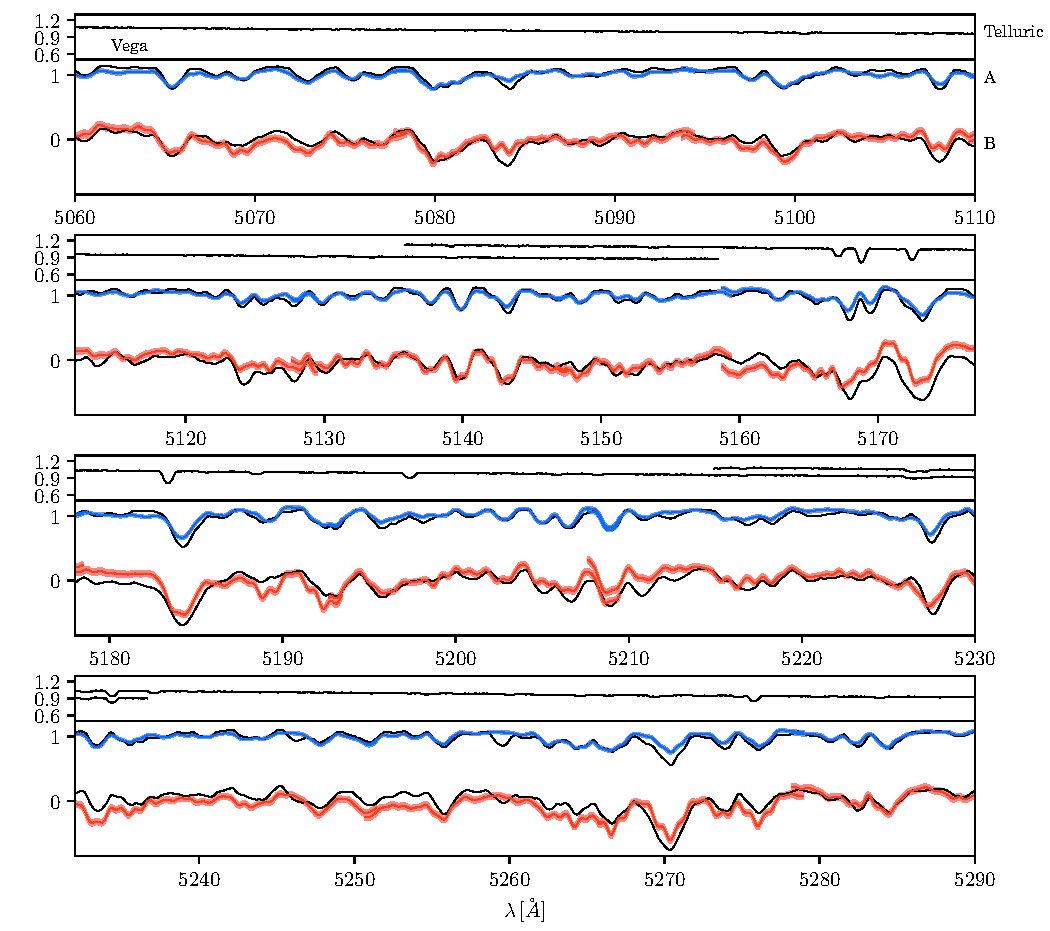
\includegraphics{disentangled-spectra.pdf}
  \figcaption{The disentangled spectra of \gw~A and \gw~B in blue and red, respectively. The top bar shows a spectrum of Vega, to demonstrate that this wavelength band is free from any telluric line contamination. The disentangled spectra have been inversely scaled by an assumed flux ratio to bring their continuum level to 1 to facilitate better comparison to the synthetic models. Disentangled spectra at the edges of echelle orders may appear jagged (e.g. $\sim 5160\,$\AA). In this figure, we have assumed $f_B / f_A = 0.43$. The overplotted synthetic models for the primary and secondary stars have stellar parameters $T_\mathrm{eff} = 6000\,$K, $\log g = 3.0\,$ dex, $v \sin i = 40\,\kms$ and $T_\mathrm{eff} = 5000\,$K, $\log g = 3.0\,$ dex, $v \sin i = 35\,\kms$, respectively.
  \label{fig:disentangled}}
  \end{center}
\end{figure*}


\subsection{Joint Radial Velocity and Disk Constraints on Individual Component Masses} \label{sec:joint}

In this section, we combine the double-lined spectroscopic binary constraints with the constraints on the total disk mass to infer the individual stellar masses of the \gw\ system without referencing the \citet{berger11} astrometry. We construct a joint likelihood function with the following five parameters: $M_\mathrm{A}$, $M_\mathrm{B}$, $M_\mathrm{C}$, $i_\mathrm{inner}$, and $i_\mathrm{outer}$.
The double-lined radial velocity constraints are sufficiently captured by the summary statistics $M_\mathrm{A} \sin^3 i_\mathrm{inner}$, $M_\mathrm{B} \sin^3 i_\mathrm{inner}$ and $M_\mathrm{C} \sin i_\mathrm{outer} / (M_\mathrm{tot} / M_\odot)^{2/3}$ and the covariances between them, which are well represented by a multivariate Gaussian distribution.\footnote{Note that we do not use additional constraints on $q_\mathrm{inner}$ or other derived parameters, as this would amount to double-counting the radial velocity points in the fit.} The disk constraint on the total stellar mass $M_\mathrm{tot}$ is well-represented by a Gaussian, as well.
We enforce flat priors on the stellar masses and geometrical priors on the inclinations. We use the ensemble sampler MCMC \citep{goodman10,foreman-mackey13} with 20 walkers to explore the posterior for 50,000 iterations, burn 25,000 iterations, and assess convergence by ensuring the Gelman-Rubin statistic \citep{gelman14} is $\hat{R} < 1.1$ for all parameters.

\begin{deluxetable}{lcc}
\tablecaption{Joint constraints on stellar masses and orbital inclinations \label{table:component_masses}}
\tablehead{\colhead{Parameter} & \colhead{RV + astrometry} & \colhead{RV + disk}}
\startdata
$M_\mathrm{A}$ [$M_\odot$] & $3.09_{-0.59}^{+0.13}$ &  \\
$M_\mathrm{B}$ [$M_\odot$] & $1.49_{-0.28}^{+0.07}$ &  \\
$M_\mathrm{C}$ [$M_\odot$] & $0.69_{-0.17}^{+0.89}$ &  \\
$i_\mathrm{inner}$ [deg] & $36.7_{-0.8}^{+3.1}$ &  \\
$i_\mathrm{outer}$ [deg] & $48_{-29}^{+29}$ &  \\
\enddata
\tablecomments{The RV + astrometry values are replicated from Table~\ref{tab:elements} for comparison purposes. We note that we are not able to infer the absolute inclination of the stellar orbits directly from the radial velocity data, so there is in fact an alternate solution for the RV + disk results that yields $i_\mathrm{alt} = 180^\circ - i$. This solution would be inconsistent with the astrometric results, however, so we opt to report the solutions with $i \geq 90^\circ$.}
\end{deluxetable}

\begin{figure}[ht!]
\begin{center}
  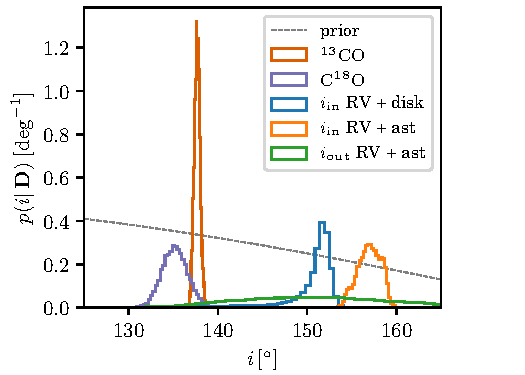
\includegraphics{incl_posterior.pdf}
  \figcaption{The inclination posteriors on the disk inclination, inner stellar orbit (A - B), and outer stellar orbit (AB - C), as determined from various joint fits. Because $i_\mathrm{out}$ is essentially unconstrained by the RV + disk analysis, we leave it off the plot for aesthetic reasons. The geometric prior on inclination (uniform orientation of orbits in 3D space) is shown as a thin grey dotted line.
  \label{fig:incl_posterior}}
  \end{center}
\end{figure}

This analysis produces the following non-symmetric posteriors on the individual component masses and orbital inclinations, summarized in Table~\ref{table:component_masses}. Although the RV + disk analysis is only able to constrain the inclination of the stellar orbits and not the position angle as well (as in the astrometric fit), there is still evidence that the stellar orbital plane is misaligned by the disk. If the inferred orbital inclinations are different, then this sets a lower limit on the total mutual inclination between the orbits (i.e., the angle between the angluar momentum vectors of the stellar orbit and that of the disk). Even if the inclinations were inferred to be the same, if the position angles were different, the orbits would be misaligned. However, if the inclinations are not the same, then the orbits are misaligned. To highlight these findings, we overplot our newly derived constraints on the disk inclination and the stellar orbits in Figure~\ref{fig:incl_posterior}.


At the lowest inclinations (nearest to edge-on, $i = 90^\circ$) are the measurements for the disk in \thirteen\ and \eighteen. This is commensurate with the disk inclination measurements from \citet{fang17}, and so we consider these results to be robust. Next, we show the inferred inner inclination from the joint RV + disk mesaurements. The outer inclination is essentially unconstrained by the RV + disk fit. The fact that the RV + astrometric fit is inconsistent with this, tells us that perhaps there is unknown systematics affecting the fit.

We show that this misalignment is probable without needing to invoke the astrometric fits. There is a small range of inclinations that overlap. And, for those to indeed overlap, would require photospheric properties which are inconsistent with our analysis. (To be detailed in next section).

% Also note that combining all of these would just result in tighter constraints on the components. But given the mis-match of the astrometric points, we claim this RV + disk analysis as our main conclusion (our data, too).


\subsection{Photometric Analysis}
Using the Lomb-Scargle (LS) periodicity search algortithim \citep{Lomb76,Scargle82} within the VARTOOLS analysis package \citep{Hartman:12}, we searched for periodic variability in the high cadenced KELT observations. Specifically, we remove the eclipses shown in Table \ref{tab:eclipses} from the KELT data and searched for a periodic signal from 1.1 to 100 days. The top two periods we recover are 74.798 and 2.931 days. See Figure \ref{figure:phased} for the phase-folded lightcurves. Additionally, we remove the KELT observations and phase the $V$-band observations from ASAS, ASAS-SN, and Maidanak to our derived orbital periods of 241.79 and 4121.12 days. We find no convincing coherent signal at the $\sim$242 days but the photometric observations phased to the $\sim$4121 day period show a coherent sinusoidal variability with a peak-to-peak amplitude of $\sim$0.15 mag.


\todo{Discussion of possible occulter size and orbital radius}
%
% Also see: http://arxiv.org/pdf/1608.07291v1.pdf
%
\begin{deluxetable}{rrrrl}
\label{tab:eclipses}
\tablecaption{V-band Photometric Eclipse Catalog\label{table:eclipses}}
\tablehead{\colhead{Start} & \colhead{End} & \colhead{Duration} & \colhead{Depth} & \colhead{Telescope} \\
\colhead{JD} & \colhead{JD} & \colhead{days} & \colhead{mmag} & }
\startdata
2447043 & 2447056 & 13 & 600 & Maidanak \\
2447153 & 2447179 & 26 & 300 & Maidanak \\
2447418 & 2447435 & 17 & 450 & Maidanak \\
2447809 & 2447824 & 15 & 130 & Maidanak \\
2448137 & 2448162 & 25 & 300 & Maidanak \\
2448545 & 2448586 & 41 & 150 & Maidanak \\
$\geq$2450399 & $\leq$2450414 & $\leq$15 & 300 & Maidanak \\
2452184 & $\geq$2452209 & $\geq$ 25 & 750 & Maidanak \\
2454445 & 2454502 & 57 & 100 & ASAS \\
2455507 & 2455535 & 28 & 60 & KELT \\
2456212 & 2456248 & 36 & 110 & KELT \\
2456709 & 2456742 & 33 & 150 & KELT \\
2456989 & 2457032 & $\leq$43 & $\geq$250 & KELT \\ % Nov 28th, 2014
\enddata
\end{deluxetable}


\section{Discussion} \label{sec:discussion}

% With the disk-based and radial velocity constraints now in place, we shift discussion to the photospheric properties of the stars, age of the system. Then, we use these constraints to discuss the dynamic inner environment, given rise to by the triple nature of the system, including the quasi-periodic nature of the photometric eclipses and pulsed accretion. Finally, we discuss the system architecture in context of other triple systems and possible formation mechanisms.

\subsection{The Age and Photospheric Properties of the GW Ori Stars}

% First, discuss Keivan's compilation of the SED, and how he did the fitting, and what we are using as our estimates for Teff priors and total system luminosity.


% Discuss/rehash how the spectroscopic constraints give us a rough estimate of V-band flux ratio and effective temperatures

% Report on the fit for age, Teff, M_A, M_B, M_C and L_star using the MIST models. As constraints, we have total luminosity, H-band flux ratio, total stellar mass, and broad posteriors on T_eff1 and T_eff2. Compare these masses as inferred to that using the joint RV + disk results. They seem to be similar.

% Figure: Use posteriors on Teff, L to plot A, B, and C on an HR diagram, which we'll reference.

% Update Figure 14 (the Teffs and f_ratios as a function of age) using the mean best predictions for the stellar properties.

Pre-main sequence evolutionary models are commonly used to infer the mass and age of young stars using measurements of their photospheric properties. We perform this exercise for \gw~A and evaluate the consistency of the model predictions with our measured dynamical mass. Due to the lingering uncertainties in the orbital constraints and thus the individual component masses, rather than evaluating the consistency of the pre-Main Sequence model predictions compared to our measured fundamental properties, instead we simply use the pre-Main Sequence models to guide discussion about the individual component properties and assess consistency.

We adopt the luminosity constraints and extinction values of \obj\ as determined by \citet{fang14}: $L = 48 \pm 10\,L_\odot$ and $A_\mathrm{V} = \todo{XX}$.

% List the models.
We evaluate the concordance of the following pre-main sequence models: \citet{choi16} models, \citet{dotter08}, \citet{tognelli11}, and \citet{siess00}. We cannot test the \citet{baraffe15} models because they do not include models with sufficiently massive stars.

We evaluate the model predictions in a Bayesian manner, following the approach in \citet{jorgensen05,rosenfeld12b,czekala15a}. The models deliver (among other quantities) the photospheric properties as a function of stellar mass and age,
e.g., $T_\mathrm{eff}(M_\ast, \tau)$ and $L(M_\ast, \tau)$.
The posterior probability distribution is found by evaluating the consistency of the model predictions for a given \{$M_\ast$, $\tau$\} with the measured photospheric properties by \citet{fang14}, multiplied by any priors on  \{$M_\ast$, $\tau$\} (in this case, flat)\footnote{Our code used to perform this analysis is available under an MIT open source license here: \url{https://github.com/iancze/ScottiePippen}}.
The resulting posterior probability distributions are shown in Figure~\ref{fig:PMS} and are listed in Table~\ref{table:agreement}. In general, all four models make similar predictions about GW~Ori~A, $\langle M_A \rangle = 3.9 \pm 0.3\,M_\odot$ and $\langle \tau \rangle = 0.6 \pm 0.3\,$Myr. We assess the probability of consistency between the model-predicted mass and our dynamical mass by evaluating $p(M_\mathrm{model} = M_\mathrm{dyn}) = \int_0^\infty p_\mathrm{model}(M) \, p_\mathrm{dyn}(M) \, \mathrm{d}M$. For most models, the predicted stellar mass is significantly less than our measured dynamical mass, $M_A = 4.40 \pm 0.18\,M_\odot$, and is consistent only at the $2\sigma$ level. \todo{Notably, the value of $M_A$ predicted by our joint radial velocity and astrometric fit ($M_A = 3.72 \pm 0.32\,M_\odot$) is in complete agreement with the model predictions.} As mentioned by \citet{fang14}, \gw~A is likely at an earlier evolutionary stage than Herbig Be stars, although it will eventually become one.

\citet{berger11} modeled the H-band visibilities of the \gw\ system measured by the IOTA/IONIC3 interferometer, and measured the positions of all three \gw\ components and their flux ratios. Their mean H-band flux ratios (computed as the weighted mean of all measurements) are $f_B/f_A = 0.57 \pm 0.05$ and $f_C/f_A = 0.23 \pm 0.01$. In Figure~\ref{fig:evolution}, we plot the ratio of effective temperatures and the computed flux ratios in Bessell I band and 2MASS H band. Bessell I roughly corresponds to the reddest echelle orders of the TRES spectrograph that we used to search for companion spectral lines. These flux ratios are generally very small and provide an explanation for why we were unable to detect secondary or tertiary spectral lines in our searches. Moreover, this means that the excess H-band flux of the B and C components is likely due to the presence of a circumstellar disk or accretion signatures above the photospheric emission of these stars, as \citet{berger11} speculated. \gw\ thus presents itself as an ideal candidate for long-term high resolution infrared radial velocity monitoring to detect spectral lines from the secondary and tertiary.

% Discuss the conversation about how massive GW Ori is by Berger 11, Fang 14, and Fang 17. Our revised mass is lower.

\begin{figure}[htb]
\begin{center}
  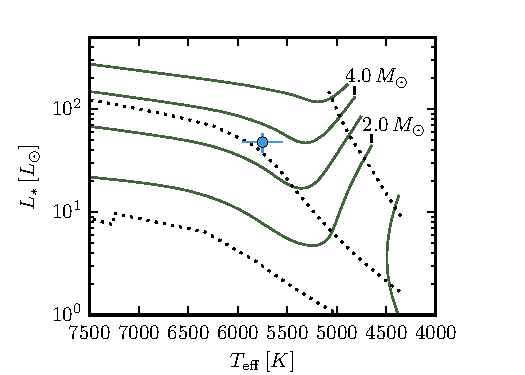
\includegraphics{tracks.pdf}
  \figcaption{An HR diagram showing all three stars.
  \label{fig:PMS}}
  \end{center}
\end{figure}


\begin{figure}[htb]
\begin{center}
  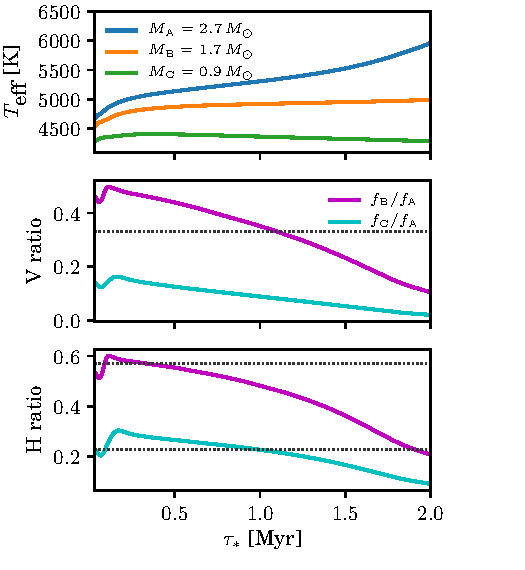
\includegraphics{evolution.pdf}
  \figcaption{Relative photospheric properties of the GW~Ori stellar components as a function of age, assuming they are coeval, predicted by the MIST pre-main sequence evolutionary models. \emph{top}: The cool effective temperature of GW~Ori~A indicates that it must be a very young star ($\tau < 5\,$Myr). The nominal age of GW Ori as predicted by the MIST models is labeled as a vertical dashed line. \emph{middle and bottom}: the predicted flux contrasts in Bessell I band and 2MASS H, respectively.
  \label{fig:evolution}}
  \end{center}
\end{figure}


\subsection{The dynamic center of the GW~Ori system} \label{sec:inner disk}

% 1 paragraph discussing that GW Ori is a triple system with misaligned orbits, photometric eclipses, and possible CO excess in the center.

% Is the tertiary in the disk? What is the effect of the tertiary orbit on the disk, regarding inclination?
% Photometric eclipses. This complicated tertiary flow may also contribute to photometric eclipses seen in the optical.

% How does this relate to the pulsed accretion population? UZ Tau E, TWA 3A, DQ Tau?
% Brief discussion of pulsed accretion and linking to UZ Tau, TWA3, DQ Tau, etc..

% How does this relate to the Dipper population?

% Najita's blended fundamental emission peaks \citep{najita03}, while \citet{bast11} suggest that these might actually be the blended profiles of emission originating from physically distinct regions. In this case, perhaps individual circumstellar disks around the A and B stars. Or, the CO fundamental emission is consistent with with radius at the inner edge of the circumtriple disk, cleared by the C component. The tertiary star makes a complicated accretion flow than that studied for other well-known binaries \citep[e.g., DQ~Tau;]{artymowicz94,mathieu97}.


\subsection{The \gw\ triple system in context}

% probably quite young, making \gw\ an extremely interesting system to study in the context of star and planet theories about formation, migration, and stability.


% Discussion about the disk, its size, mass, etc. in context
% GW~Ori disk mass in context of \citet{andrews13}.
% Note Eisner 12, Sheehan and Eisner 14 discuss high disk masses in Taurus class I (younger sources).
% Mann 15 also suggests young sources have more massive disks. NGC 2024.

% Discussion of misaligned disks
% KH 15D
% TWA 3 (Hen 3-600)
% Kellog et al \citep{kellog17}. Circumbinary disk in a triple system. Disk is likely to be misaligned with both the inner orbital plane and the outer orbital plane.

%  Toomre analysis: Is the disk stable today?
% Given the large disk mass and the massive components, we investigate whether whether the disk is Toomre stable today and whether it is possible that the stars formed from disk fragmentation due to gravitational instability. We estimate Toomre's Q parameter using
% \begin{equation}
% Q = \frac{c_s \Omega}{\pi G \Sigma} = \sqrt{\frac{k_\mathrm{B} M_\mathrm{tot}}{\pi^2 \mu m_\mathrm{H} G}} \sqrt{\frac{T(r)}{r^2 \Sigma^2(r)}}
% \end{equation}
% For the range of disk parameters determined from our CO fitting, the minimum value is $Q \approx 10$, which occurs far in the outer disk, at $r \sim 300\,$au. So, the disk is not currently undergoing disk instability. \todo{How do our estimates of the disk mass from the dust compare to the large values determined by \citet{mathieu91,mathieu95}?}


%% Switch to discussion about stellar properties, and orbital properties in context

% 1 sentence summary about the basics of the system (period, mass, mass ratio)
% It is now clear that \gw\ is a massive triple star system ($M_\mathrm{tot} = 5.5\,M_\odot$), hosting a massive and large disk ($M_\mathrm{disk} \gtrsim 0.5\,M_\odot$, $r_c \sim 250\,\mathrm{au}$). Given the observed composite spectrum (G8) and inferred component masses it is also

% While the ratio between the outer orbital period and the inner orbital period is smaller than in many hierarchical systems, it is not an outlier among triple systems.  In a detailed analysis of higher-order multiple systems, \citet{tokovinin97} found that the ratio $P_\mathrm{long} / P_{\rm short}$ in almost all systems was greater than 10, presumably reflecting which orbits are stable.  In GW Ori, this ratio is 16.

% (Tokovinin has an updated catalog on his website with about twice as many systems as in the CDS version from this paper, but it would be non-trivial to figure out how to remake the above plot.  Not sure it's necessary.)

% Among late B star primaries (which GW Ori A will be on the main sequence), 13\% of systems have multiplicity of three or higher \citep{eggleton08}; this fraction is roughly constant across spectral types B--G.

% Bate 2012 on his big fragmentation simulation: ``In particular, despite the fact that no objects form closer than $\approx 10$ au from each other, at the end of the calculation there exist 21 binary systems and one triple system with separations $<10$ au.''

% In his simulations, of the triples that form, the orbits are misaligned with each other (though three are $\leq 6$ degrees, and 8 out of 9 are $\leq 36$ degrees).

% Bate:  ``Observations also indicate that eccentricities $e < 0.1$ are rare for periods greater than $\approx$ 100 d (separations $\gtrsim$ 1 au). Raghavan et al. (2010) find no binaries with $e < 0.1$ and orbital periods greater than 100 d, though they do find that the outer orbits of two triples and one quadruple have $e < 0.1$. Duquennoy \& Mayor (1991) and Raghavan et al. (2010) also find that the upper-eccentricity envelope is dominated by components of triple systems, possibly due to the action of the Kozai mechanism (Kozai 1962).''
%
% Important for us to see what constraints we have on eccentricity of the orbits. The low eccentricity of the outer orbit is interesting in context of other systems.


%% Given the disk properties in context, and stellar properties in context, can we make any conclusions about how the system formed?
% How did the various components form?

% Fragmentation can be due to cooling or accretion. Highly variable accretion can force disks up to the fragmentation threshold, where binarity is a frequent outcome. Consensus that GI-formed objects will become brown dwarfs or stellar binary companions \citep{kratter10}, due to moderate disk temperatures and active accretion, which will grow these GI formed objects to higher masses.
%
% \citep{stamatellos09} BD formed in massive disks, but disks should be short lived. (Prediction for GW Ori lifetime?) Clearly disks are older than a few thousand years (their prediction). Predict lower mass objects are ejected by dynamical interactions. Disk fragmentation is a robust mechanism for brown dwarf formation. Again, most objects formed in disk grow to brown dwarf or hydrogen burning masses.
%
% \citep{forgan13} objects that form via GI, 90\% are above deuterium burning limits. Population synthesis model. GI then tidal downsizing is not principal mode of planet formation, but is primary means of forming brown dwarfs and low mass stars at large $a$.
%
% \citep{offner10}.
% Turbulent fragmentation is dominant channel for binary formation for \emph{low mass} stars. Is disk accretion ever so violent that it induces disk fragmentation? The fact (assumption?) that everything is coplanar and low eccentricity are expected from fragmentation from a single disk. Conclude that binaries are formed via turbulent core fragmentation (not disk). Disks are not massive enough to have gravitational instability in the disk. \citet{offner10} cite Howe \& Clarke 2009 for a review of observations.
%
% \citet{tokovinin97} finds that the distribution of mutual inclinations of the orbits in triple systems is inconsistent both with complete alignment of the inner and outer orbits, but also with independent inclinations of the two orbits.  However, we should note that this is for a population of much older systems, in which significant dynamical evolution could have occurred, particularly for the shorter-period systems.  The fact that GW Ori appears to have roughly-aligned, circular inner and outer orbits (!! does it?  to be confirmed) is suggestive of formation of one or both companions from the massive disk surrounding the system.  (Wild speculation here.)
%
% Speculation from \citet{berger11} about whether the stellar system is actual stable.



% Need some comments on KH 15D (Chiang and Murray-Clay 2004, Capelo 2012). Disk around binary is misaligned by 10 - 20 degrees.

% Ian's notes from Tokovinin 2017.
% Statistics of the angle between the orbital momentum vectors in hierarchical triples with known inner visual or astrometric orbits.  For triples with outer projected separation < 50 au, the average misalignment is 20 degrees, wheras orbits wider than 1000 au are not aligned.

% Notes that accretion of gas with randomly aligned angular momentum at the epoch of star formation can cause misaligned triples.
% \citep{tokovinin17}.

% Ian's notes from Zanazzi et al. 17., Martin et al. 17
% This may be worth a small citation regarding how misalignments can occur, but given the moderate eccentricity of GW Ori, I'm not really sure it's that applicable.
% Circumbinary disks around eccentric binaries (e > 0.5), with moderately misaligned initial inclinations (> 40 degrees) can be driven towards severe polar misalignement, where the disk is perpendicular to the binary orbit.


% Discussion of Elias 27, Perez
% Disks can develop spiral arms. Motivaton for future observations in scattered light.



\section{Summary and Conclusions} \label{sec:summary}

\begin{itemize}
\item Derived a dynamical mass for GW Ori
\item Derived a new SB2 orbit for the stars, and disentangled spectra
\item Compared the mutual inclinations for the disk and the stellar orbits
\item Evaluate the concordance between stellar properties and PMS models
\item Published lightcurve w/ eclipse analysis
\item Placed system in context of triple systems
\item Placed system in context of dippers
\end{itemize}

\acknowledgments
IC acknowledges support from the Smithsonian Institution for the production of this manuscript. IC acknowledges helpful conversations with Maxwell Moe about GW Ori and related systems.  SA acknowledges the very helpful support provided by the NRAO Student Observing Support program related to the early development of this project.  This paper makes use of the following ALMA data: XX  ALMA is a partnership of ESO (representing its member states), NSF (USA), and NINS (Japan), together with NRC (Canada) and NSC and ASIAA (Taiwan), in cooperation with the Republic of Chile.  The Joint ALMA Observatory is operated by ESO, AUI/NRAO, and NAOJ.  This research made extensive use of the Julia programming language \citep{julia12} and Astropy \citep{astropy13}.

\bibliographystyle{yahapj.bst}
\bibliography{GWOri.bib}

% \allauthors

\end{document}
